\documentclass[12pt,a4paper,oneside]{book}
\usepackage[italian]{babel}
\usepackage[UTF8]{inputenc}
%\usepackage[latin1]{inputenc}
\usepackage{amsmath}
\usepackage{geometry}
\usepackage{amsthm}
\newtheorem{thm}{Teorema}
\usepackage{amsfonts}
\usepackage{amssymb}
\usepackage{graphicx}
\usepackage{eso-pic}
\usepackage{setspace}
\usepackage{fancyhdr}
\pagestyle{fancy}
\renewcommand{\chaptermark}[1]{%
	\markboth{\thechapter.\ #1}{}}
\lhead{\leftmark}
\chead{}
\rhead{}
\lfoot{}
\cfoot{\thepage}
\rfoot{}
\renewcommand{\headrulewidth}{0pt}
\renewcommand{\footrulewidth}{0pt}
\newcommand{\fncyblank}{\fancyhf{}}
\newenvironment{abstract}% 
{\cleardoublepage\fncyblank\null \vfill\begin{center}% 
\bfseries \abstractname \end{center}}% 
{\vfill\null}
\usepackage{afterpage}
\newcommand\blankpage{%
	\null
	\thispagestyle{empty}%
	\addtocounter{page}{0}%
	\newpage}
\newcommand\AlCentroPagina[1]{% 
\AddToShipoutPicture*{\AtPageCenter{%
\makebox(0,0){\includegraphics%
[width=1\paperwidth]{#1}}}}}
\setlength{\parindent}{0pt}
\setlength{\parskip}{1ex plus 0.5ex minus 0.2ex}
\author{Maria Luisa Feola}
\title{Un'introduzione alle reti neurali e reti di Hopfield}

%COSE CHE SERVONO

%`` e '': sono le virgolette del TeX; non esistono, nel TeX, le virgolette semplici ( " ) come in Word; le virgolette `` nella tastiera italiana vengono ottenute con la combinazione di tasti “ALT + 96”, mentre le altre sono il segno dell'apostrofo;

%\mbox{parola} per non far staccare la parola

% \vspace{lunghezza} inserisce uno spazio verticale pari a lunghezza

%\hyphenation{parola sillabata}

% ~ ALT+126 tilde da mettere tra due parole per non farle staccare quando si va a capo
%FINE COSE CHE SERVONO


%INIZIO DI TUTTO
\begin{document}


%FRONTESPIZIO
%\AlCentroPagina{IMMAGINI/Frontespizio}\thispagestyle{empty} 
\blankpage

%DEDICA
\begin{flushright}
	%\newpage
	\null\vspace{\stretch{1}}
	\thispagestyle{empty}
	\textit{A mia madre, la mia vera insegnante.}
	\vspace{\stretch{2}}\null
\end{flushright} 
%FINE DEDICA


%FRASE
\begin{flushright} 
	\newpage
	\null\vspace{\stretch{1}}
	\thispagestyle{empty}
	\textit{Se non puoi passare attraverso una montagna, giraci intorno; \\ se non puoi girarci intorno, passaci sopra;\\ se non puoi passarci sopra, siediti un attimo \\e chiediti se raggiungere l'altro lato sia davvero così importante.\\ \vspace{0.5cm} Se lo è comincia a scavare una galleria.\\ \vspace{0.5cm} (Anonimo)}
	\vspace{\stretch{2}}\null
\end{flushright} 
%FINEFRASE

\clearpage
%INDICE
	\tableofcontents\addtocontents{toc}{\protect\thispagestyle{empty}}
	\thispagestyle{empty}
%FINE INDICE

%INTRODUZIONE
\newgeometry{top=3cm}
\chapter*{Introduzione}
\addcontentsline{toc}{chapter}{Introduzione}

Il presente lavoro ha come oggetto le reti neurali artificiali ed in particolar modo il funzionamento delle reti di Hopfield.\\
Il primo capitolo si apre con una breve presentazione storica sulle origini delle reti neurali artificiali e partendo da una breve esibizione del neurone biologico e della sua attività, sono mostrate le analogie che quest'ultimo ha con le reti artificiali. \\
Costituite da un insieme di interconnessioni e neuroni artificiali, tali reti sono realizzate ispirandosi ai meccanismi ed alle strutture delle reti neurali biologiche ed il loro obiettivo è la riproduzione delle attività tipiche del cervello umano. Pertanto in tale capitolo è illustrato il modello matematico del neurone artificiale, nonché il processo di attivazione di un generico neurone, esibendo le funzioni di attivazione comunemente utilizzate e le principali architetture attraverso cui possono essere modellate le reti artificiali.\\
Nel secondo capitolo è dedicato ampio spazio alle fasi di apprendimento delle reti artificiali ed ai paradigmi attraverso i quali una rete può apprendere, sottolineando il tratto caratteristico del sistema nervoso a cui tali reti neurali si rifanno, ovvero la capacità di acquisire esperienza da esempi del mondo reale. Dunque è contemplata la fase di addestramento di tali strutture e sono illustrati i maggiori processi di apprendimento e le attività che una rete può svolgere in base alla tipologia del problema che deve risolvere.\\
Infine è presentato un esempio di apprendimento supervisionato attraverso il percettrone elementare, proposto da Frank Rosenblatt nel 1958 e che risulta essere ancora oggi la forma più semplice di rete neurale.\\
Il terzo capitolo è incentrato sulle reti di Hopfield, una tipologia di rete neurale artificiale nota per il suo utilizzo nella costruzione di memorie associative. La rete può essere intesa come un sistema dinamico non lineare che evolve verso una configurazione stabile. Tale stabilità risulta essere strettamente legata ad una funzione interna che rappresenta l'energia totale del sistema e pertanto sono riportati cenni sul concetto di stabilità di Lyapunov e di funzione di Lyapunov.\\
Il capitolo si conclude con l'esibizione di una rete di Hopfield nel caso discreto e nel caso continuo e con delle osservazioni che concernono i limiti inevitabili legati a questa struttura.

%FINE INTRODUZIONE
\restoregeometry


%INIZIO DEL PRIMO CAPITOLO
	
\chapter{ Presentazione delle reti neurali }
	
	
% CAPITOLO 1 PARAGRAFO 1
	\section{Cenni storici ed origini}
		Le reti neurali artificiali, dall'inglese \textit{Artificial Neural Network (ANN)}, e la conseguente computazione neurale, sono state costruite ispirandosi ai sistemi neurali biologici con l'obiettivo di simulare il comportamento di questi ultimi, riprodurne la struttura e le funzioni basilari.\\
		Una definizione semplice e formale di tali strutture è fornita dall'inventore del primo neurocomputer, il Dr. Robert Hecht-Nielsen che le definì come: \\
		
		\textit{«...a computing system made up of a number of simple, highly interconnected processing elements, which process information by their dynamic state response to external inputs»}\\
		\textit{(da Neural Network Primer: Parte uno, Maureen Caudill, 1989)}\\
		
		Tradotto in italiano \\
		\textit{«... un sistema di calcolo costituito da una serie di semplici elementi di elaborazione, altamente interconnessi, che elaborano le informazioni attraverso il loro stato dinamico rispondendo agli input esterni.»}\\
		
		Le basi per lo studio di tali reti furono poste dallo psichiatra Warren McCulloch e del matematico Walter Pitts, i quali riuscirono a riprodurre una rete neurale utilizzando semplici circuiti elettrici collegati tra loro. Questa collaborazione portò alla luce l'analogia esistente tra le reti neurali e la macchina di Turing ed in tal modo si capì che qualsiasi operazione eseguita da una rete neurale poteva essere eseguita anche da un computer. Le reti che furono prodotte risultavano essere automi a stati finiti in grado di realizzare la logica delle proposizioni e di formulare ipotesi sulla natura dei meccanismi cerebrali come un programma per computer. Il frutto di tale lavoro fu reso noto nel 1943 con la pubblicazione del libro ``\emph{A logical calculus of the ideas immanent in nervous activity}'', nel quale fu schematizzato un combinatore lineare a soglia con dati binari multipli in entrata e un singolo dato binario in uscita.\\
	    McCulloch e Pitts riuscirono quindi a presentare il modello di neurone formale dimostrando che reti formate da tali neuroni riuscivano a computare funzioni della logica del primo ordine.\\
	    Un punto di svolta per lo studio delle reti neurali si ebbe successivamente alla pubblicazione del lavoro dello psicologo Donald Hebb, ``\emph{The Organization of Behavior}'' nel 1949. Hebb trovò un'interconnessione tra la psicologia del comportamento umano e la fisiologia del sistema nervoso, offrendo così un grande contributo alla teoria sull'apprendimento associativo. Tale teoria  risultò essere alla base dei metodi di apprendimento delle reti neurali e si fonda sulla nota legge di Hebb: \textit{«Se un neurone A è abbastanza vicino ad un neurone B da contribuire ripetutamente e in maniera duratura alla sua eccitazione, allora ha luogo, in entrambi i neuroni, un processo di crescita o di cambiamento metabolico per cui l'efficacia di A nell'eccitare B viene accresciuta»}.\\
	    Il decennio che va dagli anni cinquanta agli anni sessanta fu totalmente influenzato dalla legge di Hebb che vide che numerosi gruppi di ricerca condurre esperimenti e test sulle funzionalità del cervello fino a porre le basi per la nascita dell'intelligenza artificiale (AI).\\
	    Nel 1958 Frank Rosenblatt introdusse il primo schema di rete neurale che designò con il termine ``\textbf{\emph{perceptron}}'', in italiano percettrone, allo scopo di fornire un'interpretazione dell'organizzazione generale dei sistemi biologici attraverso un modello mirato all'analisi di funzioni in forma matematica. Il percettrone fu il primo modello di apprendimento supervisionato, costituito da uno strato di ingresso ed uno di uscita in grado di discriminare gli ingressi in due insiemi linearmente separabili.\\
	    Il percettrone risultò essere un modello più efficace rispetto a quello binario di McCulloch e Pitts, poichè i suoi pesi sinaptici erano variabili e quindi in grado di apprendere.\\
		Nonostante l'iniziale successo di tale modello e l'interesse mostrato dalla comunità scientifica, tale rete neurale non risultò abbastanza potente; le reti a due strati basate sui percettroni avevano limiti operativi, non riuscivano cioè a risolvere tutte le classi di problemi, in particolare quelli non caratterizzati dalla separabilità lineare delle soluzioni come ad esempio l'operatore \emph{XOR}.\\
		Solo negli anni ottanta, con il matematico Paul Werbos, si superarono i limiti del percettrone di Rosenblatt.  Werbos introdusse uno o più livelli intermedi all'interno delle reti neurali creando una classe chiamata  ``\textbf{\emph{Multi-Layers Perceptron}}'' ovvero percettrone multistrato, il cui metodo di addestramento principale era l'\emph{error backpropagation}, l'algoritmo di retropropagazione dell'errore che permetteva la modifica sistematica dei pesi delle connessioni in modo da rendere la risposta della rete quanto più vicina a quella desiderata.\\
		Tale algoritmo proposto nel 1986 da David E.Rumelhart, G. Hinton e R. J. Williams consentì di superare le problematiche legate al percettrone di Rosenblatt e permise di risolvere il problema della separabilità non lineare delle soluzioni, rendendo quindi possibile calcolare la funzione XOR e segnando il definitivo rilancio delle reti neurali.
		
		
% CAPITOLO 1 PARAGRAFO 2		
	
	\section{Analogie con il sistema nervoso ed applicazioni}
	
		Come accennato nel paragrafo precedente, una rete neurale è un sistema computazionale costruito basandosi sui processi biologici naturali il cui obiettivo è la riproduzione delle attività tipiche del cervello umano, ad esempio la comprensione del linguaggio, la percezione di immagini, il riconoscimento di forme ecc.  \\
		In altre parole lo scopo di una rete neurale artificiale è l’emulazione del sistema nervoso animale in particolar modo di quello umano. Quest'ultimo presenta numerose caratteristiche che risultano essere idonee per la riproduzione di un sistema computazionale: esso è flessibile poiché si adatta ad ogni tipologia di situazione, è robusto, resistente, piccolo e dissipa poca energia.
		
		\begin{figure}[h]
			\centering
			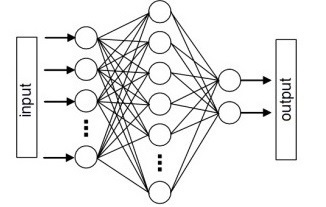
\includegraphics[width=0.5\linewidth]{IMMAGINI/esempioiniziale}
			\caption{Esempio di rete neurale}
			\label{fig:esempio}
		\end{figure}
	
		Tale riproduzione non deve essere però intesa come atta alla costruzione di un cervello artificiale. Infatti le caratteristiche delle reti neurali biologiche, riprese dalla computazione neurale artificiale, sono in esigua minoranza: gli stessi neuroni artificiali sono solo un’approssimazione dei neuroni biologici e sono in grado di riprodurre solo tre dei circa centocinquanta processi che sono tipici dei neuroni del cervello umano.
		\\Il sistema nervoso umano può essere pensato quindi come una grande struttura computazionale formata da milioni di unità fortemente interconnesse tra loro in modo parallelo riuscendo a trasformare continui input in output ragionevoli. Le reti neurali rappresentano una riproduzione significativa di tale struttura, in particolar modo degli algoritmi di apprendimento e di ottimizzazione basati su un modello \emph{connessionistico} di calcolo: le operazioni responsabili dello scambio di informazioni avvengono per mezzo dell'interazione tra le unità elementari. Esse sono sistemi altamente paralleli: fornendo i dati del problema alle unità di input, la computazione si propaga in parallelo nella rete fino alle unità di output che producono il risultato.\\
		II campo tipico di applicazione delle reti neurali è quello dell'individuazione di legami di \textbf{ingresso-uscita} all'interno di sistemi complessi in cui i dati a disposizione sono molto 
		numerosi oppure contengono poca informazione e quindi non risulta chiaro quali relazioni esistano tra le diverse variabili che caratterizzano il problema. Si tratta di campi in cui l'analisi statistica di tutte le variabili risulta difficoltosa o dispendiosa in termini di calcolo.\\ 
		Ecco un breve elenco di applicazioni note:
		
		\begin{itemize}
			\item elaborazione delle immagini (compressione e miglioramento di immagini in tempo reale);
			\item elaborazione del suono (compressione e miglioramento in tempo reale della voce e della musica, aiuti audio e protesi ecc\dots);
			\item rivelazione, verifica e identificazione di caratteri e oggetti (codici a barre, impronte digitali, firme, facce ecc\dots );  
			\item riconoscimento della voce (elaborazione di parole dettate, identificazione di persone per via vocale, selezione telefonica ecc\dots );
			\item applicazioni basate su ingressi di origine sensoriale (ingresso tattile, visivo, acustico, olfattivo);
			\item archivi (musica, video, immagini ecc\dots);
			\item sintesi e miglioramento dati (fax, grafica, cancellazione di rumore, ecc\dots);
			\item robot autonomi.
		\end{itemize}

		
%CAPITOLO1 PARAGRAFO 3		
	\section{Il neurone biologico}
		
		Per capire a fondo la connessione tra le reti neurali artificiali e le reti neurali del sistema nervoso umano e le numerose analogie che ne derivano, è bene dare una breve descrizione del secondo sistema.\\
  		Il sistema nervoso è composto principalmente dai \textbf{neuroni}, le unità fondamentali di produzione di scambi e di segnali. Ogni neurone deve adempire a cinque funzioni principali:
  		
  		\begin{itemize}
  			\item ricevere informazioni dall'ambiente esterno o interno, oppure da altri neuroni;
  			\item integrare le informazioni ricevute e produrre un'adeguata risposta in forma di segnale;
  			\item condurre il segnale al suo terminale di uscita;
  			\item trasmettere il segnale ad altre cellule nervose, ghiandole o muscoli;
  			\item coordinare le proprie attività metaboliche.
  		\end{itemize}
  	
  		\begin{figure}[h]
  			\centering
  			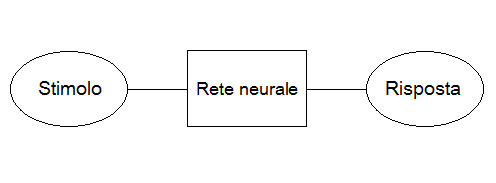
\includegraphics[width=0.6\linewidth]{IMMAGINI/Sistemanervoso}
  			\caption{Stadi del sistema nervoso}
  			\label{fig: stadi sistema nervoso}
  		\end{figure}
		
		Un neurone è formato da un corpo centrale identificato con il nome di \emph{soma} all'interno del quale è presente il nucleo, e da molti prolungamenti citoplasmatici che si distinguono in:
		 
		 \begin{description}
		 	\item[- \emph{dendriti}], organizzati con diramazioni ad albero che costituiscono il \emph{ramo dendritico};
		 	\item [- \emph{assone}], la cui parte finale prende il nome di \emph{bottone sinaptico}.
		 \end{description}
		 
		I dendriti ricevono segnali dai neuroni afferenti e li propagano verso il nucleo. Viaggiando lungo i dendriti, i segnali confluiscono al corpo del neurone che, comportandosi come un centro di integrazione, li interpreta e decide se produrre un potenziale d'azione ovvero il segnale elettrico di uscita del neurone.\\ 
		L'assone conduce il segnale verso altre cellule grazie alla presenza del bottone sinaptico alla sua estremità.
		La maggior parte dei terminali sinaptici contiene una sostanza chimica specifica, detta \emph{neurotrasmettitore}, che viene liberata in risposta a un potenziale d'azione che percorre l'assone.\\
		Il punto di connessione tra il terminale di un neurone ed il dendrite di un altro costituisce una struttura altamente specializzata che prende il nome di \emph{sinapsi} e che risulta quindi essere la responsabile delle interazioni.\\ 
		 
		  \begin{figure}[h]
		 	\centering
		 	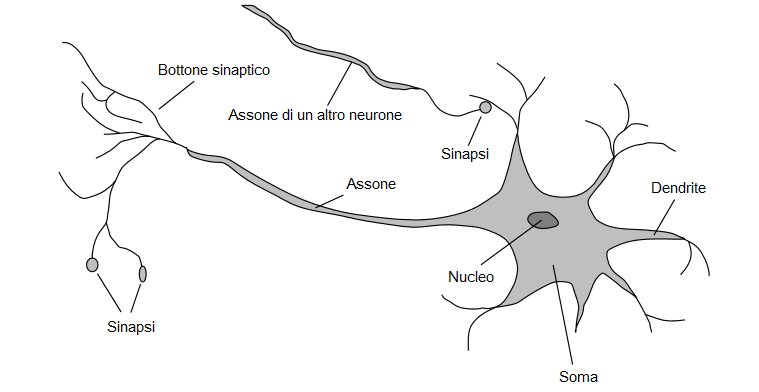
\includegraphics[width=0.7\linewidth]{IMMAGINI/neuron}
		 	\caption{Neurone biologico}
		 	\label{fig:neuron}
		 \end{figure}
		 
	 	 Nel sistema nervoso sono presenti circa $10^{11}$ cellule nervose connesse strettamente tra loro attraverso numerosi collegamenti che nel loro insieme vanno a formare la rete neurale. L'attività neurale è quindi l'attività di reti di neuroni che trasportano l'informazione ed ha come risultato finale l'emergere di sequenze significative di segnali.\\
	 	
	 	
% CAPITOLO 1 PARAGRAFO 4	
	\section{Modello del neurone artificiale}
		
		La breve illustrazione del sistema neurale umano nel paragrafo precedente suggerisce uno schema per delineare l'organizzazione delle reti neurali artificiali: queste ultime sono formate da un elevato numero di unità computazionali, che possono essere equiparate ai neuroni umani, capaci di eseguire una somma pesata. Tali unità sono collegate tra loro attraverso delle connessioni, così come le sinapsi collegano i neuroni nella rete umana. \\
		Consideriamo una generica unità $j$ costituita da $n$ canali di ingresso $x_{1}, x_{2}, ... ,x_{n}$.
		Gli input provenienti da strati precedenti o direttamente dall'esterno entrano nel neurone tramite tali canali.

		\begin{figure}[h!]
			\centering
			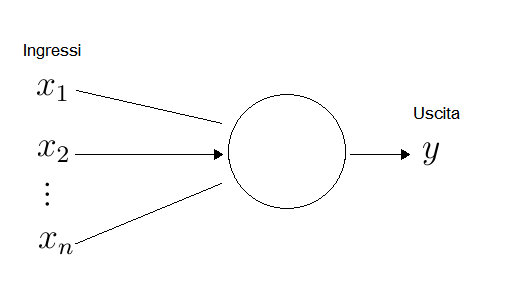
\includegraphics[width=0.7\linewidth]{IMMAGINI/palla1}
			\caption{Canali di ingresso in un neurone}
			\label{fig:palla1}
		\end{figure}
		
		Sulle connessioni sono presenti dei \emph{pesi sinaptici} $w_{i}$, numeri reali che denotano l'\emph{efficacia sinaptica}, ovvero la forza della connessione. Se $w_{i}>0$ il canale è detto \emph{eccitatorio}, se $w_{i}<0$ il canale è \emph{inibitorio}.\\
		I segnali in entrata, pesati dalle rispettive sinapsi, sono convogliati nel \emph{soma} del neurone artificiale all'interno del quale vengono sommati producendo una combinazione lineare così definita:
		
		\begin{equation} 
			\label{eqn:net} 
				$$ \begin{center} $\displaystyle\sum\limits_{i=1}^n w_{i}x_{i}$ \end{center}$$
		\end{equation} 
		
		La somma pesata degli ingressi viene indicata con la parola \emph{net} ed il segnale con cui il neurone trasmette la sua attività all'esterno è calcolato applicando una \emph{funzione di attivazione} $\varphi$ che limita l'ampiezza dell'output; si assume per comodità che le ampiezze degli output appartengono all'intervallo $[0,1]$ oppure $[-1,1]$. \clearpage
		
		\begin{figure}[h!]
			\centering
			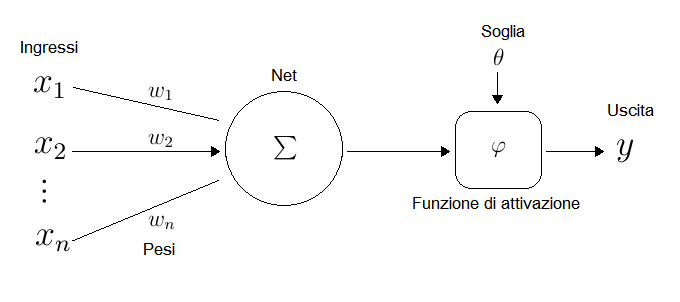
\includegraphics[width=0.8\linewidth]{IMMAGINI/palla2}
			\caption{Modello neurone}
			\label{fig:palla2}
		\end{figure}
		
	
		Il modello neuronale include anche un valore \emph{soglia} che ha l'effetto, a seconda della sua positività o negatività, di aumentare o diminuire il valore in ingresso alla funzione di attivazione.\\
		L'output finale sarà allora:
		
		\begin{equation}
			\label{eqn:output1} 
				$$\begin{center} $\displaystyle y= \varphi (\sum\limits_{i=1}^n w_{i}x_{i})$  \end{center}$$
		\end{equation}
	
		E se indichiamo con $\theta$ il valore di soglia, la~\eqref{eqn:output1} diventerà:
		\begin{equation}
			\label{eqn:output2}
				$$\begin{center} $\displaystyle y= \varphi (\sum\limits_{i=1}^n w_{i}x_{i}-\theta)$  \end{center}$$
		\end{equation}
		
		Interpretando la soglia come il peso associato ad un ulteriore canale di ingresso $x_{0}$, e quindi $w_{0}=\theta$, potremmo anche scrivere:
		
		\begin{equation}
			\label{eqn:output3}
				$$\begin{center} $\displaystyle y= \varphi (\sum\limits_{i=0}^n w_{i}x_{i})$ \end{center}$$
		\end{equation}
		
		\clearpage
		Il modello finale sarà
		
		\begin{figure}[h!]
			\centering
			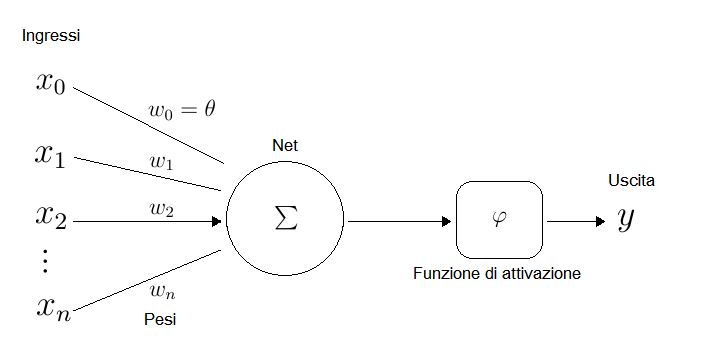
\includegraphics[width=1\linewidth]{IMMAGINI/palla3}
			\caption{ Modello neurone con soglia }
			\label{fig:palla3}
		\end{figure}
		
		L'effetto di un segnale $ x_{i} $ sul neurone è quindi uguale al prodotto 
		$w_{i}$ $\cdot$ $x_{i}$ dove $w_{i}$ è il peso attribuito alla sinapsi corrispondente ed il potenziale di attivazione è dato dalla somma algebrica dei prodotti di tutti i segnali di ingresso e dei valori dei pesi corrispondenti.\\
	 	Schematizzando ed individuando il neurone artificiale come l'unità di calcolo fondamentale della rete neurale, gli elementi base che lo rappresentano sono:
		
		\begin{itemize}
			\item un insieme di connessioni;
			\item un sommatore;
			\item una funzione di attivazione;
			\item un valore di soglia.
		\end{itemize}
		
		
% CAPITOLO 1 PARAGRAFO 5		
	
	\section{Attivazione di un neurone e funzioni di attivazione}
		
		Nelle reti neurali si può avere una \emph{attivazione asincrona} in cui i neuroni si attivano uno per volta ed un'{attivazione sincrona} in cui tutti i neuroni si attivano contemporaneamente. L'attivazione di un neurone dipende solo dall'informazione ricevuta ed è indipendente dalle operazioni svolte dagli altri nodi. La funzione di attivazione determina il tipo di risposta che un neurone è in grado di emettere. Definisce, quindi, l’uscita di un neurone in funzione del livello di attivazione. L'uscita può essere un numero reale, un numero reale appartenente ad un intervallo, oppure un numero appartenente ad un insieme discreto.\\
		Gli step per l'attivazione di un neurone sono:
		
		\begin{enumerate}
		\item i valori di input arrivano al neurone e vengono combinati con i relativi pesi; 
		\item i prodotti risultanti vengono sommati e tale somma viene confrontata con un valore di soglia che dipende dalla funzione di attivazione del neurone;
		\item se la somma supera il valore di soglia, il neurone si attiva inviando output sulle connessioni pesate in uscita, altrimenti viene inibito.
		\end{enumerate}
	
		Esistono varie tipologie di funzioni di attivazione, le principali sono: funzioni a soglia, funzioni lineari, funzioni lineari a tratti, funzione sigmoide.
		
		\subsection{Funzione a soglia}
		
		Imponendo $a=\sum\limits_{i=0}^n w_{i}x_{i}$, il valore di uscita di un neurone assunto é:
		
		\begin{equation}
		\label{eqn:sistemafunzioneasoglia} 
		$$\begin{center} 
				$\displaystyle y=\varphi(a)=$
					$\begin{cases}
						1 \hspace{0.8cm}se\hspace{0.1cm} a \geq 0 \\
						0 \hspace{0.8cm}se\hspace{0.1cm} a < 0
					\end{cases}$
			\end{center} $$
		\end{equation}
	
		Se si tralascia il contributo dell'ingresso $x_{0}$ dal livello di attivazione e si ha
		quindi $a=\sum\limits_{i=1}^n w_{i}x_{i}$, si avrà:
		
		\begin{equation}
		\label{eqn:sistemafunzioneasoglianosoglia} 
			$$ \begin{center} 
				$\displaystyle y=\varphi(a)=$
					$\begin{cases}
						1 \hspace{0.8cm}se\hspace{0.1cm} a \geq \theta \\
						0 \hspace{0.8cm}se\hspace{0.1cm} a <\theta 
					\end{cases}$
			\end{center} $$
		\end{equation}
		
		\clearpage
		I rispettivi grafici saranno
		
		\begin{figure}[h]
			\centering
			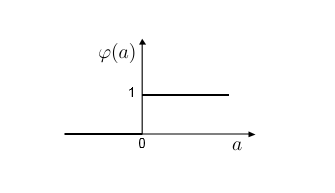
\includegraphics[width=0.95\linewidth]{IMMAGINI/asoglia}
			\caption{ Funzione di attivazione a soglia }
			\label{fig:asoglia}
		\end{figure}
		
		A volte è opportuno che la funzione di attivazione assuma valori tra $–1$ e $+1$ ed in questo caso la funzione a soglia che diviene la ben nota \emph{funzione segno} è ridefinita così : 
	
		\begin{equation}
			\label{eqn:sistemafunzionesegno} 
				$$ \begin{center} 
					$\displaystyle y=\varphi(a)=$
						$\begin{cases}
							1 \hspace{1.1cm}se\hspace{0.1cm} a>0 \\
							0 \hspace{1.1cm}se\hspace{0.1cm} a=0 \\
				    		-1 \hspace{0.8cm}se\hspace{0.1cm} a<0
						\end{cases}$
				\end{center} $$
		\end{equation}
	
		
		\subsection{Funzione lineare e funzioni lineare a tratti}
	
		Se $a=\sum\limits_{i=0}^n w_{i}x_{i}$, una funzione lineare è di questo tipo:
	
		\begin{equation}
		\label{eqn:sistemafunzionelineare} 
			$$ \begin{center} 
					$ \displaystyle y=\varphi(a)=a$
			\end{center} $$
		\end{equation}
		
		\clearpage
		Un esempio di funzione di attivazione lineare a tratti è:
	
		\begin{equation}
		\label{eqn:sistemafunzionelineareatratti} 
			$$ \begin{center} 
				$\displaystyle y=\varphi(a)=$
					$\begin{cases}
						1 \hspace{1.86cm}se\hspace{0.1cm} a \leq -0.5 \\
						a+0.5 \hspace{0.8cm}se\hspace{0.1cm} -0.5<a<0.5\\
						0 \hspace{1.86cm}se\hspace{0.1cm} a\geq0.5 
					\end{cases}$
			\end{center} $$
		\end{equation}
		
		Rappresentandole si ha
		\begin{figure}[h]
			\centering
			\includegraphics[width=1\linewidth]{"IMMAGINI/lineare e lineare a tratti"}
			\caption{Funzione lineare(a sinistra), funzione lineare a tratti (a destra)}
			\label{fig:linearelineareatratti}
		\end{figure}
		
		\subsection{Funzione sigmoide}
	
		La funzione sigmoide appartenente alla famiglia di funzioni continue non lineari ed è tra le più utilizzate.\\
		Tra queste funzioni riportiamo la \emph{funzione logistica} così definita:
	
		\begin{equation}
			\label{eqn:sigmoide} 
			$$ \begin{center} 
				$\displaystyle y=\varphi(a)=\dfrac{1}{1+e^{-a}}$
				\end{center} $$
		\end{equation}
	
		imponendo sempre $a=\sum\limits_{i=0}^n w_{i}x_{i}$.\\
		\clearpage
		Essa assume questa forma
		\begin{figure}[h]
			\centering
			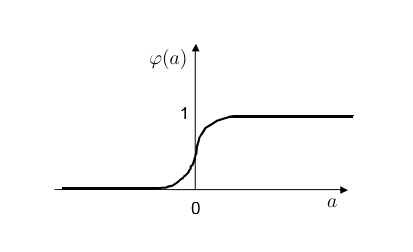
\includegraphics[width=0.6\linewidth]{IMMAGINI/sigmoide}
			\caption{ Funzione sigmoide }
			\label{fig:sigmoide}
		\end{figure}
	
	
%CAPITOLO 1 PARAGRAFO 6	
	\section{Architettura di una rete neurale}
		
		L'architettura di una rete neurale artificiale è caratterizzata da:
		
		\begin{itemize}
			\item numero di strati di sinapsi;
			\item numero di neuroni presenti nell'\emph{input layer} ovvero lo strato di ingresso;
			\item numero di neuroni nell'\emph{output layer}, lo strato di uscita.
		\end{itemize}
	
		Le reti neurali si suddividono principalmente in due grandi classi: le reti \emph{feedforward} e le reti \emph{feedback} o \emph{ricorrenti}. 
		Si ha inoltre un'altra tipologia di reti che sono le \emph{reti completamente connesse}.\\
		
		\begin{figure}[h]
			\centering
			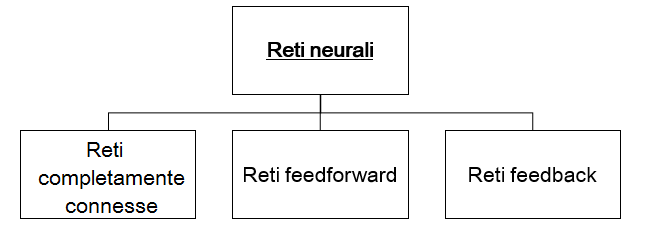
\includegraphics[width=0.75\linewidth]{IMMAGINI/diagrammareti}
			\caption{ Suddivisione delle reti neurali}
			\label{fig:diagrammareti}
		\end{figure}
		
		\underline{\emph{Reti completamente connesse}}\\
		Nelle reti completamente connesse ogni neurone è connesso con tutti gli altri. Le connessioni tra i neuroni sono bidirezionali e possono essere rappresentate per mezzo di una matrice quadrata $W$ di dimensione pari al numero di neuroni. Un suo generico elemento $w_{i,j}$ rappresenta il peso della connessione tra il neurone $i$ ed il neurone $j$.  
		
		\begin{figure}[h!]
			\centering
			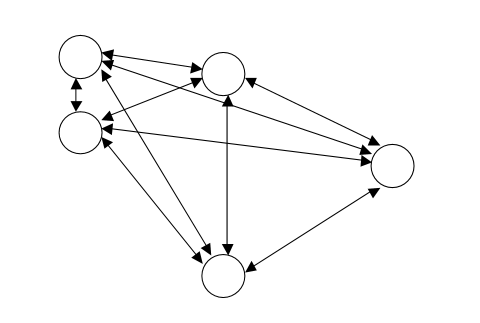
\includegraphics[width=0.5\linewidth]{IMMAGINI/completamenteconnesssa}
			\caption{ Rete completamente connessa}
			\label{fig:completamenteconnesssa}
		\end{figure}
		
		\underline{\emph{Reti feedforward a strati}}\\
		In queste reti i segnali viaggiano dallo strato di ingresso verso lo strato di uscita e pertanto vengono anche chiamate \textbf{reti feedforward}. Nelle reti stratificate non esistono connessioni tra i neuroni all'interno di uno stesso strato, nè tra neuroni di strati non limitrofi. Ogni neurone in un generico strato è connesso con tutti quelli dello strato successivo ed i neuroni dello strato di ingresso hanno come unico compito quello di trasmettere i segnali ricevuti allo strato successivo, all'interno di essi non avviene alcuna computazione.\\
		Le reti feedforward a strati si distinguono in base al numero di strati che presentano, numero che dipende dallo specifico problema che si intende risolvere.\\ 
		- \emph{Reti feedforward ad uno strato} : questa è una forma semplice di reti a strati. Il segnale nella rete si propaga in avanti senza cicli, non ci sono connessioni che tornano indietro e nemmeno connessioni trasversali nel layer di output.\\
		- \emph{Reti feedforward a più strati }: le reti a più strati sono anche dette \textit{reti multilivello }, in inglese \textbf{\textit{}Multi-Layer Perceptron, MLP}. Tra l'input layer e l'output layer sono presenti uno o più strati di neuroni nascosti, si parla quindi di \textit{\textit{hidden layers}} Nelle MLP non esistono connessioni nè tra neuroni di uno stesso strato nè tra neuroni di strati non limitrofi. Ogni strato ha connessioni entranti dal precedente strato e uscenti in quello successivo, quindi la propagazione del segnale avviene in avanti in modo aciclico e senza connessioni trasversali.\\
		Tali reti vengono utilizzate per superare problemi che possono sorgere nella discriminazione dei segnali: attraverso i neuroni nascosti si ottengono delle rappresentazioni interne dei segnali di input che consentono il riconoscimento di forme più complesse, facilitando il compito della rete. 
		Nonostante tutto l’aggiunta di ulteriori strati nascosti non ottimizza le abilità di discriminazione della rete; questo è possibile solo se la funzione di attivazione è non lineare (una rete multistrato a neuroni lineari è sempre riconducibile ad una rete con due soli strati).
		
		\begin{figure}[h]
			\centering
			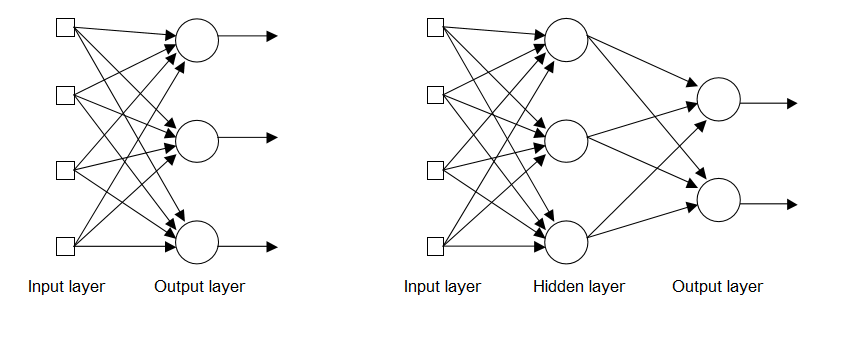
\includegraphics[width=0.95\linewidth]{IMMAGINI/unostrato}
			\caption{Rete ad uno strato (a sinistra), rete multilivello (a destra)}
			\label{fig:multistrato}
		\end{figure}
	
		\underline{\emph{Reti ricorrenti}}\\
		Una rete neurale ricorrente (RNN) si distingue dalle precedenti nel fatto che è ciclica. Il sistema è dinamico, le unità di output sono connesse con quelle intermedie e con quelle di input, si ha una \emph{retroazione}. Dato un determinato stimolo la risposta della rete ricorrente non viene dettata soltanto dai caratteri strutturali della rete stessa, come si verifica nella rete feedforward, ma varia in funzione del precedente contesto in cui si è manifestato lo stimolo. L'output non è determinato solo dall'input, ma anche da una \emph{cronologia} di input che fornisce una forma di memoria a breve termine. Queste reti sono adatte per dati strutturati temporalmente ed hanno anche la possibilità di avere un’attività in assenza di una stimolazione input poiché gli impulsi che viaggiano sulle vie ricorrenti possono essere sufficienti a mantenere il sistema in attività.
	
%FINE PRIMO CAPITOLO%



%INIZIO DEL SECONDO CAPITOLO%
	
\chapter{L'apprendimento delle reti neurali}
	
	
%CAPITOLO 2 PARAGRAFO 1
	\section{Addestramento e generalizzazione}
		
		Per costruire una rete neurale efficiente un passo fondamentale è individuare un \textbf{insieme di apprendimento} ed un \textbf{algoritmo di apprendimento}.\\
		Per insieme di apprendimento si intende una collezione di esempi chiamata \textbf{training set} dai quali la rete può attingere per raggiungere lo scopo per il quale è stata progettata; per algoritmo, invece, un procedimento che permetta di prelevare le informazioni dall'insieme di apprendimento e di fissare dei parametri che vengano poi modificati attraverso operazioni iterative interfaccianti con l'ambiente.\\
		L’apprendimento avviene sempre grazie ad un certo numero di esempi prelevati dal mondo reale ed opera in due fasi distinte: 
		
		\begin{itemize}
			\item Fase di apprendimento o addestramento nota come \textbf{learning} o \textbf{training};\\
			\item Fase di generalizzazione nota come \textbf{recall}.
		\end{itemize} 
		
		Durante la fase di learning si cerca di far imparare alla rete tutte le informazioni contenute nel training set ottenendo un modello che verrà poi utilizzato nella fase di generalizzazione per analizzare nuovi ingressi.\\  
		L’architettura della rete neurale gioca un ruolo fondamentale per l’efficienza nella fase di apprendimento. Non bisogna però immaginare che con l'aumentare del numero di unità cresca il potere computazionale della rete. Infatti, in tal caso, ci si troverebbe di fronte ad una situazione di \emph{overfitting}, un adattamento forzato della rete dato che risulterebbe avere un numero eccessivo di parametri rispetto al numero di esempi forniti. Questa situazione tende a far diminuire la capacità della rete di generalizzare su nuovi esempi originando una sorta di principio di indeterminazione dell'apprendimento che può essere affrontato con la limitazione del numero degli ingressi.\\ 
		Per \textbf{generalizzazione} di una rete si intende la sua capacità di fornire le risposte appropriate a pattern di input che non sono mai stati incontrati. Essa risulta essere un punto di forza delle reti neurali e dipende dal numero di unità nascoste, dai pesi sinaptici e dal numero di training record.\\
		Una rete neurale ``generalizza bene" se la mappa input/output che essa genera è corretta per esempi di test mai presentati in fase di training (si assume che gli esempi di test siano tratti dalla stessa popolazione usata per generare il training set). In questi termini essa produce mappature input/output corrette anche se l’input è lievemente differente dagli esempi usati in fase di training; se però la rete viene addestrata con troppi esempi, si rischia che quest'ultima memorizzi il training set trovandosi nella condizione di \emph{overtraining}. \\ 
		Per avere una struttura ottimale della rete dal punto di vista della capacità di generalizzazione una guida adatta è il \textbf{Principio di Occam}, che suggerisce molto sulla complessità delle reti e sulla loro adeguatezza e che in relazione a queste ultime, può essere enunciato nel seguente modo:
		
		\textit{``Date due reti che soddisfano l'insieme di apprendimento, la rete di minore complessità è quella che si comporta meglio su esempi non visti, cioè ha la migliore capacità di generalizzazione."}\\ 
		
		
	
% CAPITOLO 2 PARAGRAFO 2
	\section{Paradigmi di apprendimento}	
		Le reti neurali si ispirano al tratto caratteristico del sistema nervoso, ovvero la capacità di acquisire esperienza da esempi del mondo reale: per questo, oltre che di apprendimento, si parla di \emph{addestramento} delle reti neurali attraverso dei \textit{paradigmi di apprendimento}.\\
		I paradigmi di apprendimento si suddividono in:
		
		\begin{itemize}
			\item \emph{apprendimento \textbf{supervisionato} }
			\item \emph{apprendimento \textbf{non supervisionato}}
		\end{itemize}
	
		\underline{Apprendimento supervisionato}\\
		Tale paradigma presuppone un \emph{training set} cioè un set di esempi nel quale sono presenti coppie del tipo $(x_{k},y_{dk})$ dove la prima variabile indica il $k$-esimo ingresso e la seconda la $k$-esima uscita desiderata. Con $y_{k}$ si indica l'uscita reale e la si confronta con l'uscita desiderata: l'obiettivo è modificare i pesi affinché si minimizzi la differenza tra le due uscite. Il training set iniziale viene proposto ripetutamente finché $y_{k}\approx y_{dk}$, ovvero l'uscita reale sia il più simile possibile a quella desiderata, il tutto modificando i pesi in base alla legge di apprendimento scelta.\\
	
		\begin{figure}[h]
			\centering
			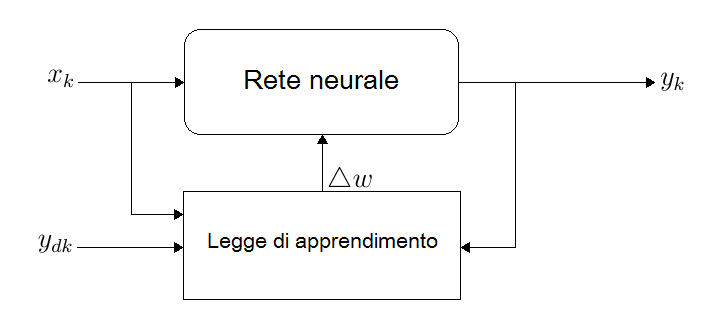
\includegraphics[width=0.8\linewidth]{IMMAGINI/supervisionato}
			\caption{ Apprendimento supervisionato }
			\label{fig:supervisionato}
		\end{figure}
		
		\underline{Apprendimento non supervisionato}\\
		
		Nell'apprendimento non supervisionato la rete modifica i pesi autonomamente, si auto-organizza. Viene fornito solo il training set senza precisare le uscite.\\
	
		\begin{figure}[h]
			\centering
			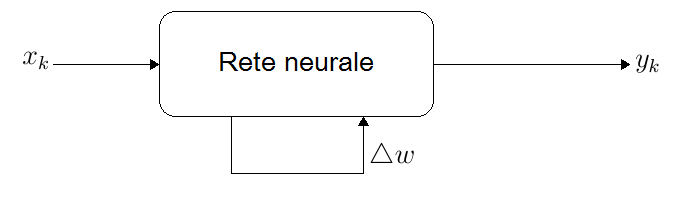
\includegraphics[width=0.7\linewidth]{IMMAGINI/nonsupervisionato}
			\caption{ Apprendimento non supervisionato}
			\label{fig:nonsupervisionato}
		\end{figure}
	
	

% CAPITOLO 2 PARAGRAFO 3
	\section {Processi di apprendimento}
		 
		 L’addestramento è un processo ad hoc dipendente dallo specifico problema trattato. Riportiamo alcuni processi comunemente usati.\\
		 
		 
		 \subsection{Delta rule}
		 
		 Con regola delta, o \emph{delta rule}, si intende un apprendimento con correzione dell’errore. 
		 Siano:\\
		 $\displaystyle\overline{x}_{k}=[x_{1}, x_{2}, ..., x_{n}]^{T}$ il vettore $k$-esimo degli ingressi,\\ 
		 $\displaystyle\overline{W}_{k}=[w_{1}, w_{2}, ..., w_{n}]^{T}$ il vettore dei pesi al $k$-esimo ingresso,\\
		 e siano $y_{k}$ ed $y_{dk}$ rispettivamente l'uscita ottenuta e l'uscita desiderata. Definiamo l'\emph{errore} come:
		
		 \begin{equation}  
			 $$ \begin{center} $\displaystyle \delta_{k}=y_{k}-y_{dk} $ \end{center} $$
		 \end{equation} 
	
		 Allora se consideriamo la variazione del generico vettore dei pesi $\overline{W}_{k}$ si ha che:
		 
		 \begin{equation}  
		 	$$ \begin{center} $\displaystyle \triangle\overline{W}_{k}=\eta\overline{x}_{k}\delta_{k}$ \end{center} $$
		 \end{equation}
		 
		 Il numero $\eta$ che compare nell'equazione (2.2) è compreso tra $0$ ed $1$, prende il nome di \textbf{learning rate} ed indica la velocità di apprendimento del neurone.\\
		 Questa regola modifica in maniera proporzionale solo i pesi delle connessioni che hanno contribuito all'errore.\\
		 
		 L'algoritmo è il seguente:
		 
		 \begin{enumerate}
		 	\item se $y_{k}=y_{dk}$ nessuna modifica dei pesi
		 	\item se $y_{k}\neq y_{dk}$ allora $\triangle\overline{W}_{k}=\eta\overline{x}_{k}\delta_{k}$.
		 \end{enumerate}
		 
		 
		 \subsection{Apprendimento con correzione di errore o metodo discesa del gradiente}
		 
		 Se indichiamo con $y_{k}$ una risposta generata da un segnale di stimolo $x$ in un tempo $t$ ed indichiamo con $y_{dk}$ la risposta desiderata, avremo un \emph{segnale di errore} che può essere così espresso:
		 
		 \begin{equation}
		 	$$\begin{center} $\displaystyle \delta= y_{k}-y_{dk}$ \end{center}$$
		 \end{equation}
		 
		 Tale segnale dà il via ad un meccanismo di controllo che va ad applicare una sequenza di modifiche ai pesi sinaptici del neurone interessato al fine di avvicinare la risposta ottenuta a quella desiderata.\\
		 
		 \begin{figure}[h]
		 	\centering
		 	\includegraphics[width=0.8\linewidth]{"IMMAGINI/errore"}
		 	\caption{ Apprendimento con correzione }
		 	\label{fig:errore}
		 \end{figure}
		 
		 Questo processo di ricerca dei pesi migliori si basa sulla scelta di pesi che minimizzano una funzione errore $E(\overline{W})$, costruita al variare dei pesi stessi. \\
		 Per la scelta di tali pesi si sfruttano le informazioni fornite dal gradiente locale della funzione errore costruita.\\
		 Se con $\nabla_ {w}E(\overline{W})$ indichiamo il gradiente della funzione, allora:
		 
		 \begin{equation}
			 $$\begin{center} $\displaystyle \Delta W \varpropto \nabla_ {w}E(\overline{W}) $ \end{center}$$
		 \end{equation}
		 
		 \begin{figure}[h]
		 	\centering
		 	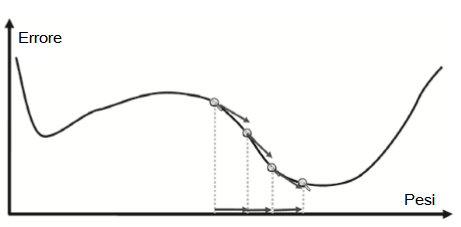
\includegraphics[width=0.8\linewidth]{IMMAGINI/gradiente}
		 	\caption{Metodo della discesa del gradiente}
		 	\label{fig:gradiente}
		 \end{figure}
		 
		 La ricerca risulta quindi essere guidata in modo proporzionale e dato che:\\
		
		\begin{equation}
		 $$\begin{center}
		 	 $\displaystyle\frac{dE(\overline{w})}{d\overline{w}}=\nabla_ {w}E(\overline{w})=( \frac{\partial E(\overline{w})}{\partial w_{1}}, \frac{\partial E(\overline{w})}{\partial w_{2}}, ... ,\frac{\partial E(\overline{w})}{\partial w_{n}} )^{T}$
		 \end{center}$$
		\end{equation}
		 
	 	si avrà:
	 	
	 	\begin{equation}
	 		$$\begin{center}
	 		   $\displaystyle\triangle\overline{W_{k}}=\eta\frac{dE(\overline{w})}{d(\overline{w})}$
	 		\end{center}$$
	 	\end{equation}
	 	
	 	Se consideriamo la $k$-esima uscita $y_{k}$ e la rispettiva uscita desiderata $y_{dk}$ ed indichiamo con $g$ la funzione di attivazione:
	 	
	 	\begin{equation}
	 		\label{eqn:coppiagradiente} 
	 			$$\begin{center} 
	 					$\displaystyle \begin{cases}
	 						y_{k}=g(net_{k})\\
	 						\delta_{k}=y_{k}-y_{dk} 	
	 					\end{cases}$
	 			\end{center} $$
	 	\end{equation}
	 	
	 	Si definisce l'\textbf{errore quadratico medio}:
	 	
	 	\begin{equation}
	 		$$\begin{center}
	 		$\displaystyle E_{k}=\frac{1}{2}(y_{k}-y_{dk})^{2}$
	 		\end{center}$$
	 	\end{equation}
	 	
		 Ma allora se consideriamo l'$i$-esimo peso del $k$-esimo input si avrà che:
		 
		 \begin{equation}
		 	$$\begin{center}
				 $\displaystyle\triangle{w_{i}}=\eta\frac{\partial E_{k}}{dw_{i}}$
		 	\end{center}$$
		 \end{equation}
		 
		 e sviluppando:
		 
		 \begin{equation}
		 	$$\begin{center}
		 	$\displaystyle\frac{\partial E_{k}}{dw_{i}}=
		 	\dfrac{\partial}{\partial w_{i}}[\frac{1}{2}(y_{k}-y_{dk})^{2}] =
		 	(y_{k}-y_{dk}) \frac{\partial (y_{k}-y_{dk})}{\partial w_{i}} =
		 	(y_{k}-y_{dk})\frac{\partial y_{k}}{\partial w_{i}} = $
		 	\end{center}$$
		 	$$\begin{center}
		 	$\displaystyle = (y_{k}-y_{dk})\frac{\partial g(net_{k})}{\partial w_{i}}=
		 	(y_{k}-y_{dk})\frac{\partial g(net_{k})}{\partial net_{k}}\frac{\partial net_{k}}{\partial w_{i}}=
		 	\delta_{k} g'(net_{k}) x_{i} $
		 	\end{center}$$
		 \end{equation}
		 	
		 	Quindi il peso $w_{i}$ sarà modificato:
		 	
		 	\begin{equation}
		 		$$\begin{center} $\displaystyle\triangle{w_{i}}=\eta\frac{\partial E_{k}}{dw_{i}}=\eta\delta_{k} g'(net_{k}) x_{i}$ 
		 		\end{center}$$	
		 	\end{equation}
		 
		 
		\subsection{Apprendimento di Hebbian}
		
		Come nella delta rule, definiamo:\\
		$\overline{x}_{k}=[x_{1}, x_{2}, ..., x_{n}]^{T}$ il vettore $k$-esimo degli ingressi,\\ 
		$\overline{W}_{k}=[w_{1}, w_{2}, ..., w_{n}]^{T}$ il vettore dei pesi al $k$-esimo ingresso,\\
		e siano $y_{k}$ ed $y_{dk}$ rispettivamente l'uscita ottenuta e l'uscita desiderata.\\
		Nell'apprendimento di tipo hebbiano viene modificato ogni valore del peso di una connessione in questo modo:

		\begin{equation}
			$$ \begin{center}
			 	$\displaystyle\triangle\overline{W}_{k}=\eta\overline{x}_{k}y_{dk}$ 
			 \end{center} $$
		\end{equation}
	
		con $\eta$ learning rate.\\
		
		I passi dell'algoritmo sono i seguenti:
		\begin{enumerate}
			\item se $y_{k}=y_{dk}$ nessuna modifica pesi
			\item se $y_{k}>y_{dk}$ allora $\triangle\overline{W}_{k}=-\eta\overline{x}_{k}y_{dk}$
			\item se  $y_{k}<y_{dk}$ allora $\triangle\overline{W}_{k}=\eta\overline{x}_{k}y_{dk}$
		\end{enumerate}
		
		
		\subsection{Apprendimento competitivo}
		 
		 Tale apprendimento si basa su una vera a propria competizione tra i neuroni di uscita di una rete neurale per attivarsi in seguito ad uno stimolo. In un certo momento $t$ può attivarsi un solo neurone che viene denominato \textbf{winners-takes-all}.\\  
		 In tale processo è importare avere quindi un meccanismo che permetta ai neuroni di competere ed un valore che indichi il limite della ``forza" di ciascun neurone.\\
		 Nella forma più semplice la rete neurale ha un solo strato di neuroni di uscita completamente connessi ai nodi di input e che possono essere connessi tra loro.
		 \clearpage
		
		 \begin{figure}[h]
		 	\centering
		 	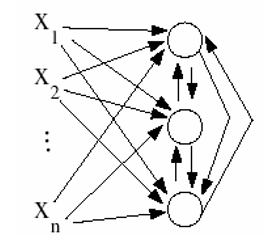
\includegraphics[width=0.4\linewidth]{IMMAGINI/competitivo}
		 	\caption{ Struttura rete con apprendimento competitivo}
		 	\label{fig:competitivo}
		 \end{figure}
		 
		 Il neurone $k$ che si attiva è quello con input netto $\nu_{k}$ più alto per un dato input $x$, con $\nu_{k}$ combinazione lineare di tutti gli input. Il suo segnale di output $y_{k}$ sarà $1$ mentre quello degli altri neuroni rimasti inattivi è $0$.
		 
		 \begin{equation}
		 \label{eqn:competitivo} 
		 	$$\begin{center} 
		 		$\displaystyle y_{k}=$
		 		$\displaystyle \begin{cases}
		 				1 \hspace{0.8cm}se\hspace{0.1cm} \nu_{k}>\nu{j} \hspace{0.6cm} \forall j,\hspace{0.2cm} j\neq k;\\
		 				0\hspace{0.8cm} altrimenti
		 			\end{cases}$
		 	\end{center} $$
		 \end{equation}
		 
		 Ora se indichiamo con $w_{k,j}$ i pesi tra il neurone $k$ e l'input $j$, supponendo che ogni neurone abbia un ammontare di peso sinaptico fisso $\sum\limits_{j} w_{kj}=1, \forall k$, il neurone che vince apprende spostando i pesi dagli input inattivi agli input attivi utilizzando tale regola:
		 
		 \begin{equation}
		 \label{eqn:competitivo} 
		 	$$\begin{center} 
		 		$\displaystyle\triangle w_{kj}=$
		 			$\begin{cases}
						\eta(x_{j}-w_{kj}) \hspace{0.8cm}se\hspace{0.1cm} il\hspace{0.1cm} neurone\hspace{0.1cm} k\hspace{0.1cm} vince;\\
		 				0\hspace{2.7cm} altrimenti
		 			\end{cases}$
		    \end{center} $$
		 \end{equation}
	
	
% CAPITOLO 2 PARAGRAFO 4	
\section{Attività di apprendimento}
		
		La scelta del paradigma di apprendimento, e quindi la metodologia di addestramento di una rete neurale, avviene in base all'attività che la rete deve svolgere ovvero il problema che deve risolvere. Le reti neurali possono essere utilizzate come \emph{classificatori} in grado cioè di riconoscere oggetti appartenenti a diverse categorie o possono essere responsabili dell'approssimazione di funzioni. Data una funzione nota per punti, di cui non si conosce la forma analitica, il compito della rete neurale è quello di approssimarla nel modo migliore possibile calcolandone il valore anche in punti diversi da quelli proposti in ingresso.\\
		
		\subsection{Associazione di pattern e memoria associativa}
		
		Per memoria associativa intendiamo un criterio di memorizzazione e recupero di informazioni attraverso l'associazione. Completamente ispirata al metodo di memorizzazione del cervello umano, consente il recupero dell'informazione sulle basi di una conoscenza parziale del suo contenuto senza conoscerne la locazione di memoria.\\
		La memoria associativa si articola in due fasi:\\
		
		\begin{itemize}
		 \item fase di memorizzazione: la rete viene addestrata per fare in modo che dei \emph{pattern}, vettori di numeri reali, vengano memorizzati ed associati;
		 \item fase di richiamo: si richiama dalla rete un pattern memorizzato a seguito della presentazione di una versione parziale o distorta di un pattern chiave. 
		\end{itemize}
	
		Le \emph{associazioni} possono essere di due forme:\\ 
		- \underline{\emph{autoassociazioni}}: generalmente utilizzate nell'apprendimento non supervisionato, la rete neurale memorizza un insieme di pattern che vengono ripetutamente presentati. Tra essi ne viene presentato in particolare uno che risulta essere distorto o in forma parziale. L'obiettivo è che la rete riconosca il pattern e ne richiami la versione completa/originale precedentemente memorizzata.\\
		-  \underline{\emph{eteroassociazioni}}: ogni pattern è associato ad un altro pattern; se $x_{k}$ è un generico pattern chiave associato al pattern memorizzato $y_{k}$, allora $x_{k}$ opera in modo tale da richiamare $y_{k}$.
		
		\subsection{Riconoscimento di pattern}
		
		Tale processo si articola in due fasi: la prima fase consiste in una sessione di addestramento in cui  alla rete vengono presentati ripetutamente un insieme di pattern specificando per ognuno la classe di appartenenza; nella seconda fase alla rete viene presentato un pattern mai mostrato precedentemente, ma appartenente ad una categoria di pattern che la rete ha memorizzato. La rete neurale sarà in grado di riconoscerne la categoria e classificare il pattern grazie ai dati precedentemente acquisiti.\\
		Il sistema è diviso in tre spazi:\\
		
		\begin{itemize}
		\item lo \emph{spazio dei dati} costituito da tutti i pattern, un generico pattern $x$ identifica un punto dimensionale di tale spazio;
		\item lo \emph{spazio delle caratteristiche} all'interno del quale sono presenti dei punti $y$;
		\item lo \emph{spazio decisionale} multidimensionale suddiviso in regioni determinate dalla rete nella fase di addestramento, ognuna delle quali è associata ad una classe.
		\end{itemize}.
		
		\begin{figure}[h]
			\centering
			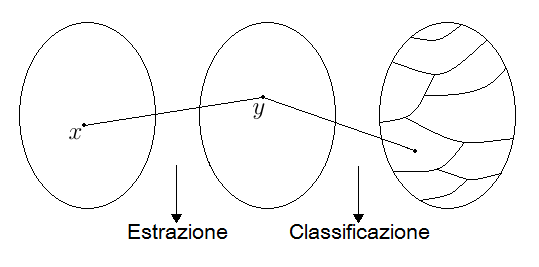
\includegraphics[width=0.8\linewidth]{IMMAGINI/classificazione}
			\caption{ Classificazione di pattern }
			\label{fig:classificazione}
		\end{figure}
		
		Il processo di riconoscimento inizia con l'estrazione delle \emph{features} ovvero le caratteristiche che un generico pattern nello spazio dei dati deve rispettare. L'\emph{estrazione} è una trasformazione che collega il pattern $x$ con un punto $y$ nello spazio delle caratteristiche. Infine un'ultima trasformazione detta \emph{classificazione} mappa dal punto $y$ ad una regione dello spazio decisionale.\\
		
		\subsection{Approssimazione di funzioni}
		
		Si prenda in esame una rappresentazione non lineare input/output descritta da $y=f(x)$ dove $x$ è l'input e $y$ è l'output e si consideri un insieme di esempi ${(x_{i},y_{i} )}$ per $i=1, 2, ..., n$. L'incognita è la funzione $f$ ed il problema consiste nel creare una rete capace di generare una rappresentazione $F$ quanto più vicina alla funzione $f$. In senso euclidiano bisogna soddisfare la condizione\\
		
		\begin{center} $\displaystyle ||F(x)-f(x)<\varepsilon|| \hspace{0,7cm} \forall x $ \end{center}
		
		dove $\varepsilon$ è un numero positivo piccolo, che risulterà essere sempre più piccolo con l'accrescere delle dimensioni e dei parametri liberi della rete. 
		
	

% CAPITOLO 2 PARAGRAFO 5		
	\section{Un esempio di apprendimento supervisionato: il percettrone elementare}
	
		\begin{figure}[h]
			\centering
			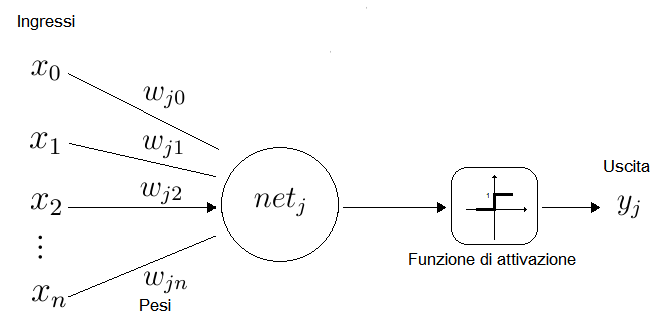
\includegraphics[width=0.85\linewidth]{IMMAGINI/perceptron}
			\caption{ Il percettrone }
			\label{fig:perceptron}
		\end{figure}	
	
		Proposto da Rosenblatt, il percettrone è la forma più semplice di rete neurale e coincide con la struttura del neurone formale. Esso è costituito da un singolo neurone in cui confluiscono più ingressi i cui pesi sinaptici sono modificabili. 
		\clearpage
		La funzione di attivazione è una funzione a gradino detta \emph{funzione di Heavside}:
		
		\begin{equation}
			\label{eqn:Heavside} 
				$$\begin{center} 
					$\displaystyle g(net_{j})=$
						$\displaystyle\begin{cases}
							1 \hspace{0.8cm}se\hspace{0.1cm} net_{j} \geq 0 \\
							0 \hspace{0.8cm}se\hspace{0.1cm} net_{j} < 0
						\end{cases}$
				\end{center} $$
	 	\end{equation}
		
	 	Il percettrone divide lo spazio di ingresso in due regione mediante l'iperpiano in $\Re^{n}$ di equazione: 
	 
	 	\begin{equation}  
	 		$$ \begin{center} $\displaystyle w_{0}+\sum\limits_{i=1}^n w_{i}x_{i}=0 $ \end{center} $$
	 	\end{equation} 
		
		ed è quindi in grado di risolvere solo problemi \emph{linearmente separabili}.\\ 
		Supponiamo di voler classificare in due classi distinte $C_{1}$ e $C_{2}$, degli oggetti rappresentati mediante punti nel piano e di sfruttare $n=2$ ingressi.\\
		Se le due classi sono linearmente separabili, l'iperpiano è una retta che funge da separatore lineare tra le due classi. Un oggetto sarà quindi classificato in base alla parte di semipiano in cui il suo punto di rappresentazione cadrà.\\
		Nel piano $(x_{1}, x_{2})$ degli ingressi della rete le classi $C_{1}$ e $C_{2}$ sono rappresentate da due semipiani separati dalla retta $x_{2}=-\frac{w_{1}}{w_{2}}x_{1}+\frac{w_{0}}{w_{2}}$ e possiamo classificare gli stimoli in questo modo:
		
		\begin{equation}
		 \label{eqn:semipiani} 
			$$\begin{center} 
				$\displaystyle\begin{cases}
						x\in C1 \hspace{0.8cm}se\hspace{0.1cm} y=1 \\
						x\in C2 \hspace{0.8cm}se\hspace{0.1cm} y=0
				\end{cases}$
			\end{center} $$
		\end{equation}
		
		
		L'apprendimento utilizzato nel perceptron è di tipo supervisionato e la learning rule attraverso i quali si modificano i singoli pesi in modo appropriato 
		\clearpage
		è la delta rule, definita in forma generale come:
		
		\begin{equation}  
			$$ \begin{center} $ \displaystyle\overline{W}_{k+1}=\overline{W}_{k}+\triangle\overline{W}_{k} $ \end{center} $$
		\end{equation} 
		
		dove $\overline{W}_{k}=[w_{1}, w_{2}, ..., w_{n}]^{T}$ è il vettore dei pesi al $k$-esimo ingresso.
		
		\begin{figure}[h]
			\centering
			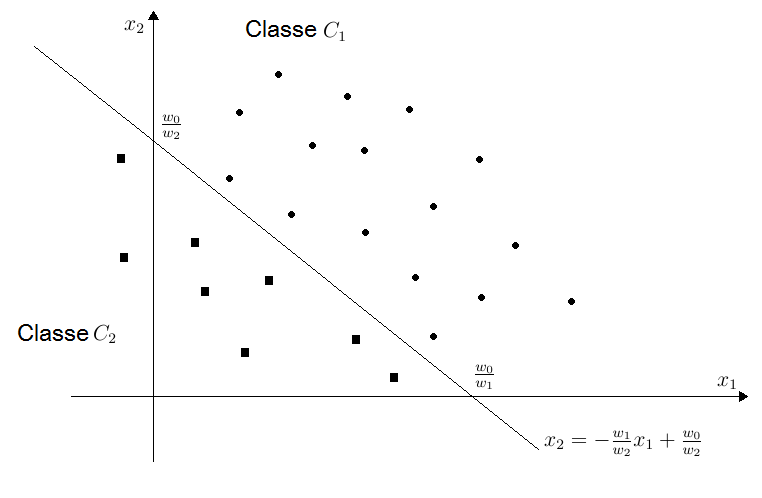
\includegraphics[width=0.9\linewidth]{IMMAGINI/rettapercettrone}
			\caption{ Separazione lineare dello spazio di ingresso di un Perceptron}
			\label{fig:rettapercettrone}
		\end{figure}
	
		I passi da eseguire sono:
		
		\begin{enumerate}
			\item {si inizializzano i pesi con valori casuali;}
			\item {si presenta un ingresso $x_{k}$ ed il valore di uscita desiderato $y_{dk}$;} 
			\item {si calcola la risposta $y_{k}$ e si aggiornano i pesi attraverso la delta rule;}
			\item {si ripete il ciclo dal passo 2 finché non si ottiene una risposta soddisfacente.}
		\end{enumerate}
	   
	   Con riferimento alla figura 2.8 si osservi che modificando i pesi $w_{1}, w_{2}, w_{0}$ si modifica la posizione e la pendenza della retta di separazione tra le due classi. Il processo termina quando la retta separa correttamente le due classi.
	
%FINE DEL SECONDO CAPITOLO




%INIZIO DEL TERZO CAPITOLO
	
\chapter{Reti di Hopfield}

%CAPITOLO 3 PARAGRAFO 1
	\section{Presentazione ed utilizzo}
	
	Le reti di Hopfield furono presentate nell'anno 1982 dal fisico John Hopfield nel suo articolo \textit{``Neural networks and physical systems with emergent collective computational abilities"}. A seguito di numerose osservazioni sulle proprietà dinamiche ed elettrochimiche dei neuroni e delle loro interconnessioni, Hopfield cercò di fare emergere gli schemi di funzionamento che erano dietro ai comportamenti biologici elementari. Il modello matematico realizzato da Hopfield dimostrò che un gran numero di semplici elementi di elaborazione possedevano capacità computazionali dal \emph{comportamento collettivo} e che tali capacità emergevano spontaneamente come conseguenza di interazioni tra le unità.\\
	Le proprietà collettive di tale modello contraddistinguono tutt'oggi le reti di Hopfield dalle restanti. Queste reti sono utilizzate principalmente nella costruzione di  memorie associative per il riconoscimento di rappresentazioni alterate ed il recupero di informazioni mancanti, imitando quindi la capacità del nostro cervello di riconoscere un'immagine anche quando questa non è esatta, risulta deformata o distorta e di riuscire a leggere parole con lettere mancanti.\\
	Tali reti sono impiegate anche:
	
	\begin{itemize}
		\item nella risoluzione di problemi d'ottimizzazione combinatoriale;
		\item nei problemi di classificazione.
	\end{itemize}

	\begin{figure}[h]
	\centering
	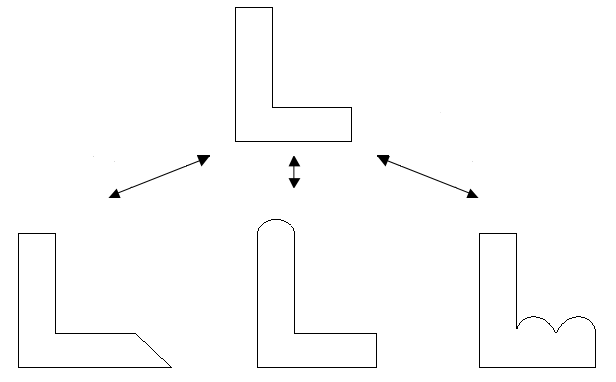
\includegraphics[width=0.55\linewidth]{IMMAGINI/riconoscimento}
	\caption{ Rete di Hopfield utilizzata come memoria associativa: l'immagine deve essere sempre riconosciuta.}
	\label{fig:riconoscimento}
	\end{figure}

%CAPITOLO 3 PARAGRAFO 2
	\section{Architettura ed aggiornamento}

	La topologia delle reti di Hopfield è completamente diversa da quella delle reti a strati. Ogni unità è collegata a tutte le altre attraverso connessioni simmetriche, in termini di pesi sinaptici si ha $w_{i,j} = w_{j,i}$ , $\forall i,j$. Sono quindi reti completamente connesse, in cui non si hanno autoconnessioni, $w_{i,i}=0$, la cui matrice dei pesi sinaptici è simmetrica con funzione di attivazione a gradino o a soglia. \\
	
	\begin{figure}[h]
		\centering
		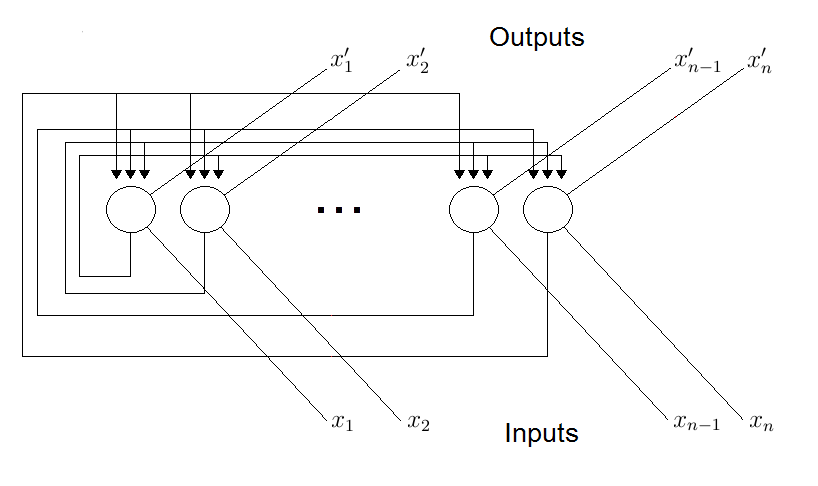
\includegraphics[width=0.9\linewidth]{IMMAGINI/hopfield}
		\caption{Esempio di una rete di Hopfield}
		\label{fig:hopfield}
	\end{figure}

	I valori di input di ogni unità sono binari e non c'è distinzione tra unità di input ed unità di output. La rete riceve i valori in entrata in numero pari alle unità che presenta per poi farli fuoriuscire dalle stesse unità una volta elaborati. In questo modello l'uscita di ogni neurone è collegata all'ingresso di tutti gli altri neuroni, formando così una topologia di rete a grafo completo unidirezionale.\\
	Nella fase di apprendimento la rete memorizza un certo numero di informazioni dette \textbf{stati stabili}, mentre nella fase operativa modifica il proprio stato sulla base dei pesi colleganti i vari neuroni: la rete itera fino a convergere su dei valori di output che rappresentano il pattern più simile all'input memorizzato dalla rete.\\
	La rete di Hopfield è una rete \textbf{ricorrente} e ad ogni rete con una simile architettura è associata una sequenza di stati. Nel nostro caso tale sequenza è rappresentata da un vettore che coincide col vettore delle attività dei neuroni. Se chiamiamo con $\overline z$ quest'ultimo vettore ed indichiamo con $\overline v$ il vettore di ingresso, $\overline v$ ha lo stesso numero di componenti di $\overline z$ e viene continuamente presentato alla rete in modo tale che ciascun neurone abbia in uscita il valore della corrispondente componente in $\overline z$. Detto $z_{n}$ lo stato della rete all'istante $t$, lo stato successivo viene calcolato come:

	\begin{equation}
	\label{eqn:hopfieldaggiornamento} 
		$$\begin{center}
			$\displaystyle z_{n+1}=Wz_{n}$
		\end{center}$$
	\end{equation}
	
	con $W$ matrice dei pesi costituita da elementi del tipo $w_{i,j}$, elemento che simboleggia il peso della connessione dal nodo $i$ al nodo $j$.\\
	In questo meccanismo di aggiornamento tutte le attività vengono aggiornate contemporaneamente e pertanto viene chiamato \textbf{aggiornamento sincrono}. Generalmente i meccanismi di aggiornamento dei neuroni sono divisi in:
	
	\begin{itemize}
		\item\textbf{aggiornamento asincrono} in cui si aggiorna un neurone alla volta;
		\item\textbf{aggiornamento sincrono} in cui tutti i neuroni sono aggiornati nello stesso istante;
		\item\textbf{aggiornamento continuo} in cui tutti i neuroni si aggiornano continuamente.
	\end{itemize}
	
	L'idea di Hopfield fu quella di attribuire alla multi-stabilità della struttura una memoria. Ogni stato stabile può essere visto come un \textbf{attrattore} per gli stati iniziali vicini ad esso, ovvero un insieme verso il quale un sistema dinamico evolve dopo un tempo sufficientemente lungo. Inizializzando quindi la rete ad uno stato iniziale, quest'ultimo evolverà verso l'attrattore. Il proposito principale è fare in modo che certi stati siano appresi come stabili e con modifiche opportune sui pesi siano resi attrattori.\\
	Abbiamo visto che il principio alla base della memorizzazione delle reti neurali è che l’informazione sia contenuta nei coefficienti di connessione. Nel modello di Hopfield si persegue tale obiettivo sfruttando la legge di Hebb, esposta nel capitolo 1 e che riprendiamo qui a grandi linee: se un’unità $j$ manda un input ad un'altra unità $i$ e se entrambe sono attive, il peso corrispondente $w_{i,j}$ deve essere rafforzato.\\
	Supponiamo di voler memorizzare il set di stati $v^ {s}$ con $s = 1, ..., n$, utilizzando la notazione in cui $0\Longleftrightarrow -1$ e $1\Longleftrightarrow 1$. \\
	I pesi delle connessioni sono fissati attraverso un apprendimento non iterativo \emph{fixed point learning}, seguendo la seguente formula: 
	
	\begin{equation}
	\label{eqn:hopfieldpesi} 
		$$\begin{center}
			$\displaystyle w_{i,j}=\sum\limits_{s}v_{i}^{s}v_{j}^{s} \hspace{0.7cm}i\neq j, \hspace{0.2cm} i,j=1,...,n $
		\end{center}$$
	\end{equation}
	
	La matrice $W$ sarà data da:
	
	\begin{equation}
	\label{eqn:hopfieldmatrice} 
		$$\begin{center}
			$\displaystyle W=v_{1}v_{1}^{T}+v_{2}v_{2}^{T}+...+v_{n}v_{n}^{T}$
		\end{center}$$
	\end{equation}
	
	Gli stati stabili risulteranno proporzionali agli autovettori della matrice dei pesi e coincideranno con i minimi di una particolare funzione che introdurremo nel prossimo paragrafo e che risulterà essere convergente proprio in essi. Questi funzioneranno pertanto come bacini d’attrazione per gli stati della rete.
	
%CAPITOLO 3 PARAGRAFO 3	
	\section {Cenni sulla stabilità}
	
	Nelle reti ricorrenti non è detto a priori che la rete riesca a convergere su uno stato stabile. Hopfield ha verificato che la stabilità del sistema delle sue reti è strettamente legata ad una funzione chiamata \textbf{funzione energia} della rete che indichiamo con $E$. Aggiungendo l'ipotesi che la matrice dei pesi sia simmetrica con diagonale principale nulla e che si lavori in una condizione di aggiornamento asincrono, Hopfield ha dimostrato che $E$ non può aumentare nel passaggio da uno stato all'altro e poiché non può raggiungere valori infinitamente negativi, lo stato della rete cesserà di cambiare in un tempo finito ed essa raggiungerà dunque uno stato stabile.\\
	La rete di Hopfield può essere quindi vista come un sistema dinamico non lineare che evolve verso una configurazione stabile e la stabilità è legata alla funzione energia.\\ 
	Prima di introdurre tale funzione, è bene dare qualche definizione in merito ai sistemi dinamici ed al concetto di stabilità vista in senso di Lyapuanov.\\
	Il modello matematico per descrivere le dinamiche di un sistema non lineare è pensato in termini di \textbf{variabili di stato}. Tali variabili rendono possibile prevedere l'evoluzione del sistema a partire da un certo istante temporale utilizzando i valori che sono associati ad esse, poiché considerati sufficienti per la previsione dell'evoluzione. Definiamo \textbf{vettore di stato}:
	
	\begin{equation}
	\label{eqn:vettoredistato} 
		$$\begin{center}
			$\displaystyle x(t)=(x_{1}(t), x_{2}(t), ..., x_{n}(t))$
		\end{center}$$
	\end{equation}
	
	un vettore contenente le variabili di stato ed in cui la variabile indipendente è il tempo $t$ mentre $n$ è l’ordine del sistema. Sfruttando tali vettori è possibile descrivere un sistema dinamico mediante un sistema di equazioni differenziali di primo ordine del tipo:
	
	\begin{equation}
		\label{eqn:eqzndifferenziale} 
			$$\begin{center}
				$\displaystyle \dfrac{d}{dt}x(t)=F(x(t))$
			\end{center}$$
	\end{equation}
	
	con $F(x)$ \textbf{funzione vettore} che applicata ad un vettore di stato $x$ ritorna un vettore che ha come $j$-esima componente $F_{j}(x_{j})$, con $F_{j}$ una qualche funzione. Tale equazione risulta descrittrice del movimento di un punto nello \textbf{spazio degli stati} $n$-dimensionale, spazio i cui punti rappresentano univocamente tutti e soli i possibili stati del sistema osservati a certi istanti $t$. Con il trascorrere del tempo il punto t descrive una curva detta traiettoria del sistema.\\
	Definiamo \textbf{stato di equilibrio} un vettore costante $\overline{x}$ verificante la seguente condizione:
	
	\begin{equation}
	\label{eqn:statodiequilibrio} 
		$$\begin{center}
			$\displaystyle F(\overline{x})=0$
		\end{center}$$
	\end{equation}
	
	Uno stato di equilibrio $\overline{x}$ è \textbf{uniformemente stabile} se:
	
	\begin{equation}
		\label{eqn:unifstabile} 
			$$\begin{center}
				$\displaystyle \forall\varepsilon>0 \hspace{0.2cm} \exists \hspace{0.1cm} \delta>0 \hspace{0.1cm} \colon \hspace{0.1cm} \Arrowvert x(0)-\overline{x}\Arrowvert <\delta \Rightarrow \Arrowvert x(t)-\overline{x}\Arrowvert < \varepsilon $
			\end{center}$$
	\end{equation}
	
	In altre parole una traiettoria del sistema può variare in un piccolo intorno dello stato di equilibrio $\overline{x}$ se il suo stato iniziale è vicino a $\overline{x}$. 
	
	\begin{thm}[Lyapunov]
	
	Lo stato di equilibrio $\overline{x}$ è stabile se in un piccolo intorno di $\overline{x}$ esiste una funzione scalare definita positiva $V(x)$ tale che la sua derivata rispetto al tempo è minore o uguale a $0$ in quella regione.
	\end{thm}

	Una funzione $V(x)$ che soddisfa queste proprietà è detta \textbf{funzione di Lyapunov} per lo stato di equilibrio $\overline{x}$.\\
	Se consideriamo un sistema dinamico, ad una sua condizione di equilibrio stabile corrisponde un minimo dell'energia posseduta dal sistema stesso come conseguenza del fatto che esso tende spontaneamente a minimizzarla. L'energia del sistema viene espressa come una funzione di Lyapunov verificante il teorema di cui sopra.
	
	
%CAPITOLO 3 PARAGRAFO 4 	
	\section {Il caso discreto e la funzione energia}
	
	La prima rete presentata da Hopfield era una rete discreta, completamente connessa, con aggiornamento asincrono e matrice dei pesi simmetrica.\\
	In questo modello ogni neurone può assumere due stati $v_i=0$ e $v_{i}=1$. Lo stato istantaneo del sistema è specificato elencando gli n valori di $v_{i}$ e lo stato di ciascun neurone ad un certo istante $t$ è determinato da una formula di attivazione binaria a soglia che modificherà i valori input seguendo questo schema: 
	
	\begin{equation}
	\label{eqn:casodiscreto} 
		$$ \begin{center} 
			$\displaystyle v_{i}^{t}=$
				$\begin{cases}
					1 \hspace{1.86cm}se\hspace{0.1cm} \sum\limits_{i\neq j} w_{i,j}v_{j}^{t-1} > \theta_{i}\\
					0 \hspace{1.86cm}se\hspace{0.1cm} \sum\limits_{i\neq j} w_{i,j}v_{j}^{t-1} < \theta_{i}
				\end{cases}$
		\end{center} $$
	\end{equation}

	dove $\theta_{i}$ è la soglia di attivazione associata al neurone $i$-esimo.\\
	In modo equivalente, se $f_{h}$ è una funzione non lineare a soglia:
	
	\begin{equation}
		\label{eqn:hopfieldpesi2} 
			$$\begin{center}
				$\displaystyle v_{i}^{t}=f_{h}(\sum\limits_{i\neq j}v_{j}^{t-1} -\theta_{1}) \hspace{0.7cm}i=1, ..., n $
			\end{center}$$
	\end{equation}
	
	Questo processo è applicato ad un'unità per volta secondo un ordine stabilito o casualmente ed iterato fino a quando la rete non raggiungerà uno stato di equilibrio che corrisponderà ai valori di output.
	
	\begin{figure}[h]
		\centering
		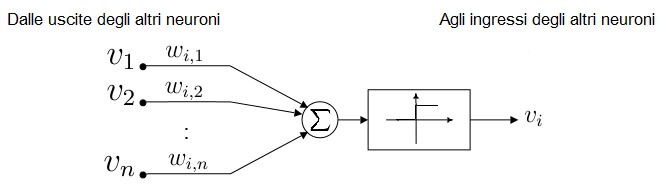
\includegraphics[width=1\linewidth]{IMMAGINI/casodiscreto}
		\caption{}
		\label{fig:casodiscreto}
	\end{figure}

	Nel paragrafo precedente abbiamo detto che la rete di Hopfield può essere vista come un sistema dinamico non lineare che evolve verso una configurazione stabile ed abbiamo accennato ad una particolare funzione, la \emph{funzione energia}. Questa risulta essere una funzione di Lyapunov definita nello spazio di stato e che viene minimizzata con l’evolvere del processo.\\
	Tale funzione assume questa forma:
	
	\begin{equation}
		\label{eqn:funzioneenergiadiscreto} 
			$$\begin{center}
				$\displaystyle E=-\frac{1}{2}\sum\limits_{i}\sum\limits_{j}w_{i,j}\hspace{0.1cm}v_{i}v_{j}+\sum\limits_{i}\theta_{i}v_{i} $
		\end{center}$$
	\end{equation}
	
	Essa è limitata inferiormente ed utilizzando un aggiornamento di tipo asincrono, risulta strettamente monotona decrescente lungo una qualsiasi traiettoria descritta dalla rete di Hopfield nello spazio di stato:
	
	\begin{equation}
	\label{eqn:strettamentemonotonadecrescente} 
		$$\begin{center}
			$\displaystyle \Delta E(t)=E(t+1)-E(t)<0 $
		\end{center}$$
	\end{equation} 
	
 	il che sta a significare che la rete evolve verso una configurazione stabile. Essa risulterà inoltre convergente ad uno stato stabile corrispondente ad un minimo locale della funzione energia.\\
	Lavorando con un aggiornamento di tipo asincrono sarà valutata solo una generica unità $k$ alla volta e può accadere che:
	
	\begin{enumerate}
		\item $v_{k}$ non cambia stato;\\
		\item $v_{k}$ cambia stato $-1\longrightarrow 1$, $1\longrightarrow -1$.
	\end{enumerate}
	
	Nel primo caso si ha $E(t+1)=E(t)$ e quindi la funzione rimane invariata.\\
	Nel secondo caso la funzione energia cambia secondo il nuovo valore $v'_{k}$. Si avrà:
	
	\begin{equation}
	\label{eqn:casodiscretodim} 
		$$\begin{center}
			$\displaystyle E(v) - E(v')= (-\frac{1}{2}\sum\limits_{j}w_{k,j}\hspace{0.1cm}v_{j}v_{k}+\theta_{k}v_{k})-(-\frac{1}{2}\sum\limits_{j}w_{k,j}\hspace{0.1cm}v_{j}v'_{k}+\theta_{k}v'_{k}) $
		\end{center}$$
	\end{equation} 
	
	Ma poiché $w_{k,k}=0$ si ha:
	
	\begin{equation}
		\label{eqn:casodiscreto2} 
			$$\begin{center}
				$\displaystyle E(v) - E(v')=-(v_{k} - v'{k})(\sum\limits_{j}w_{k,j}\hspace{0.1cm}-\theta_{k}) $
		   \end{center}$$
	\end{equation} 
	
	Osservando il secondo termine e considerando che l'unità cambia il suo stato, l'eccitazione ha un segno diverso che dipende da $v_{k}$ e $-v'_{k}$.\\
	Sfruttando la simmetricità della matrice dei pesi e il fatto che ha gli elementi diagonali nulli la (3.13) è sempre positiva, infatti:
	
	\begin{enumerate}
		\item se $v_{k}$ cambia stato e si ha $-1\longrightarrow 1$, allora $v_{k}=-1 \Rightarrow v'_{k}=1$ , da cui $-(v_{k}-v'{k})>0$;\\
		\item se $v_{k}$ cambia stato e si ha $1\longrightarrow -1$, allora $v_{k}=1 \Rightarrow v'_{k}=-1$ , da cui $-(v_{k}-v'{k})>0$ .
	\end{enumerate}

	Quindi $E(v)>E(v')$ ed allora l’energia diminuirà per ogni cambiamento. Inoltre poiché gli stati possibili sono in numero finito, la rete raggiungerà uno stato in cui l'energia non potrà diminuire ulteriormente e tale stato risulterà stabile, assicurando la convergenza della rete.
	
		\subsection{Il caso continuo}
	
		A differenza del caso discreto, la rete di Hopfield continua può assumere un numero infinito di stati sebbene sia formata da un numero finito di neuroni.\\
		Lo stato della rete all'istante $t$ è sempre rappresentato da un vettore $v$ composto dagli $n$ stati $v_{i}$ dei singoli neuroni, i cui valori sono compresi nell'intervallo reale $[{0,1}]$ se utilizziamo una notazione unipolare, $[{-1,1}]$ (notazione bipolare).
		\clearpage
		Scriviamo lo stato $v_{i}$ al tempo $t$ come segue:
		
		\begin{equation}
			\label{eqn:casocontinuostato} 
				$$\begin{center}
					$\displaystyle v_{i}(t)= k v_{i}(t-1) + \alpha \sum\limits_{j=1}^{n}w_{i,j}F_{j}(t) $
				\end{center}$$
		\end{equation} 
	
		dove $k,\alpha \epsilon [0,1]$ ed $\alpha$ è una \textbf{costante di attenuazione} mentre:
	
		\begin{equation}
		\label{eqn:casocontinuofunzione} 
			$$\begin{center}
				$\displaystyle F_{j}(t)=\dfrac{1}{1+e^{-\frac{v_{i}(t)}{T}}} $
			\end{center}$$
		\end{equation} 
	
		è una funzione di attivazione sigmoide.\\
		La funzione energia assume questa forma:
	
		\begin{equation}
			\label{eqn:funzioneenergiacontinuo} 
				$$\begin{center}
					$\displaystyle E=-\frac{1}{2}\sum\limits_{i=1}^{n}\sum\limits_{j=1}^{n}w_{i,j}\hspace{0.1cm}v_{i}v_{j}+\sum\limits_{i=1}^{n}\frac{1}{\beta}\int_{0}^{v_{i}}F_{i}^{-1}(v)dv-\sum\limits_{i=1}^{n}\theta_{i}v_{i} $
				\end{center}$$
		\end{equation}
	
		Risulta anch'essa essere una funzione Lyapunoviana e quindi anche in questo caso si ha $\displaystyle \frac{dE}{dt}\leq 0 $.
		
%CAPITOLO 3 PARAGRAFO 5
	\section{Limiti delle reti di Hopfield}
	
	L'articolo di presentazione delle reti di Hopfield riscosse grande interesse nella comunità scientifica.\\
	La rete di Hopfield risulta tutt'ora essere un robusto ed innovativo paradigma computazionale capace di fornire risposte in tempo reale. La peculiarità che desta più interesse è l'abilità di tale rete di memorizzare e recuperare i pattern in base al loro contenuto e non in base al loro indirizzo di memoria. Se alla rete viene presentato un pattern incompleto ma già memorizzato, essa opera attraverso una sequenza di stati per ottenere il pattern originale. Nonostante queste caratteristiche, il modello presenta limiti e svantaggi legati alla sua stessa natura.\\
	Tale rete è caratterizzata da un'alta complessità strutturale e la dipendenza della scelta dei pesi dal problema rende difficile la realizzazione hardware. Non ci sono garanzie sulla qualità delle soluzioni trovate ed in generale non si ottengono soluzioni ottime soprattutto per quanto concerne la memorizzazione di vettori simili in quanto si ha la probabilità di incorrere in pattern instabili. Inoltre il numero di informazioni che possono essere memorizzate risulta essere piccolo rispetto al numero di neuroni di cui la rete è composta. Se indichiamo con $n$ il numero di neuroni e con $t$ il numero di informazioni si ha:
	
	\begin{equation}
	\label{eqn:numero informazioni} 
		$$\begin{center}
			$\displaystyle t<\frac{n}{log_2 n } $
		\end{center}$$
	\end{equation}
	
	 Un altro problema sostanziale è il problema dei falsi minimi legato alla funzione energia caratteristica della rete. Abbiamo detto nei paragrafi precedenti che a partire dallo stato iniziale, l'evoluzione dinamica della rete fa diminuire la funzione energia fin quando non si arriva in uno stato che corrisponde ad un minimo della funzione e che potrebbe costituire una soluzione del problema. Durante questo processo il sistema potrebbe cadere in minimi locali non garantendo l'affidabilità del risultato. Tale risultato potrebbe essere migliorato aggiungendo rumore alle dinamiche di rete, nella speranza che il sistema evolva nonostante sia vicino ad un minimo locale. 
	
%\underline{Esempio:} In forma vettoriale possiamo scrivere:

%\begin{equation}
%\label{eqn:hopfieldpesivettoriale} 
%$$\begin{center}
%$\displaystyle\overline{w}=\sum\limits_{s} %\overline{v_{s}}\cdot\overline{v_{s}}^{T}-1$
%\end{center}$$
%\end{equation}

%Supponiamo di voler memorizzare il vettore $[+1, -1, +1, +1]$. La matrice dei %pesi verrà calcolata seguendo questo procedimento

%$$ \begin{bmatrix}
%+1\\
%-1\\
%+1\\
%+1\\
%\end{bmatrix}
%[+1, -1, +1, +1] - 
%\begin{bmatrix}
%+1 & 0 & 0 & 0 \\
%0 & +1 & 0 & 0 \\
%0 & 0 & +1 & 0 \\
%0 & 0 & 0 & +1
%\end{bmatrix} = 
%\begin{bmatrix}
%0 & -1 & +1 & +1 \\
%-1 & 0 & -1 & -1 \\
%+1 & -1 & 0 & +1 \\
%+1 & -1 & +1 & 0
%\end{bmatrix} $$
%\phantomsection 
\begin{thebibliography}{9} 
	\addcontentsline{toc}{chapter}{\refname}
	\bibitem{Bicego} Prof. Bicego Manuele, \emph{Riconoscimento e recupero dell’informazione per bioinformatica, reti neurali}
	\bibitem{Gambosi} Prof. Gambosi Giorgio, \emph{Reti neurali, note dal corso di Machine Learning}, (2010), Packt Publishing 
	\bibitem{GarretaMoncecchi} Garreta Raùl, Moncecchi Guillermo, \emph{Learning scikit-learn: Machine Learning in Python}, (2013) 
	\bibitem{Hopfield} Hopfield John Joseph, \emph{Neural Networks and Physical Systems with Emergent Collective Computational Abilities}, (1982)
	\bibitem{Labonia} Prof.ssa Labonia Laura, \emph{Storia delle reti neurali artificiali}
	\bibitem{Lazzarini} Prof.ssa Lazzarini Beatrice, \emph{Introduzione alle reti neurali}, (2015)
	\bibitem{Machiavello} Machiavello Chiara, \emph{Introduzione alle reti neurali}, (1992)
	\bibitem{Pioggia} Ing. Pioggia Giovanni, \emph{Modelli di sistemi fisiologici}, (2009)
	
 \end{thebibliography}
	
\chapter*{Ringraziamenti}
\addcontentsline{toc}{chapter}{Ringraziamenti}

Desidero ringraziare mia madre, a cui è dedicato questo lavoro di tesi, che fin dal principio mi ha sostenuto ed ha combattuto con me per il raggiungimento di questo obiettivo. Grazie per la possibilità che mi hai dato, per i valori che mi hai trasmesso e per gli insegnamenti che mi hai donato rendendomi ciò che sono oggi. Grazie per aver sempre creduto in me dandomi tutto l'amore che solo una madre può dare e grazie soprattutto per i sacrifici e per la pazienza che negli anni hai mostrato. Solo grazie al tuo sostegno ho sempre avuto l'energia per affrontare e la determinazione per proseguire, solo grazie alla tua calorosa vicinanza ho realizzato il mio progetto. Per me sei stata e sarai per sempre un esempio di madre, figlia, amica, lavoratrice, donna.\\
Ringrazio Vincenzo, compagno fedele ed amico fidato, per avermi dato forza ed entusiasmo per scalare la vetta e per essermi stato sempre vicino passo dopo passo tendendomi la mano. Grazie per avermi aiutato e sostenuto, per avermi incitato quando ero a terra, per avermi spronato quando ne avevo bisogno e per avermi rimproverato se mi lasciavo prendere da una eccessiva preoccupazione. Ti sono grata per tutti i suggerimenti ed i confronti, per aver gioito e sofferto con me, per il trasporto mostratomi che mi ha trasmesso sostegno e soprattutto coraggio. Non dimenticherò mai le tue espressioni in volto nei giorni dei miei ultimi orali mentre aspettavi l'esito e le telefonate serali prima di un esame in cui piangevo senza un motivo ben preciso. Sei stato un punto fondamentale per la mia vita negli ultimi anni e ti ringrazio per il tuo amore ed il tuo affetto.\\
Ringrazio la mia amica Maria De Riggi che ha rappresentato un pozzo di coraggio e forza nella mia quotidianità. Averti accanto in questo cammino, non solo in ambito universitario, mi ha aiutato e segnato molto e mi ha fatto scoprire una bellissima persona che non ho alcuna intenzione di perdere. Grazie per tutte le risate, le lacrime, i ricordi, le battute, i rimproveri, il calore, l'appoggio, i racconti ma soprattutto la fiducia. Grazie per aver contribuito alla mia rinascita ed aver sempre mostrato disponibilità ed accoglienza. Non dimenticherò mai questi anni passati insieme e ti sarò per sempre riconoscente per essere entrata nella storia della mia vita e per averla arricchita con la tua semplicità ed il tuo insostituibile affetto. Il ricordo di questi anni universitari passati a studiare, far sacrifici, crescere, sognare, piangere e sorridere, vincere e perdere sarà sempre legato alla tua persona. Approfitto per augurarti il meglio per il tuo prossimo ed imminente successo, sappiamo entrambe che questi nostri traguardi avrebbero avuto un altro sapore se fossero stati condivisi pienamente nello stesso giorno. Anche se il destino ha deciso di separarci, tale separazione è solo materiale, la gioia e l'orgoglio che nutriamo l'un per l'altra saranno immutati e basterà un solo nostro sguardo per cantare vittoria.\\
Ringrazio poi Antonella Letizia, amica e collega, per tutti i suggerimenti e gli incoraggiamenti nonché per il caro affetto mostratomi nel corso degli anni. La sua prontezza nell'ascoltare tutti i miei dubbi, i miei pensieri e le mie idee è stata di grande aiuto, soprattutto nell'ultimo periodo. Grazie per esserci stata e per avermi spronato nel ricercare la forza per perseguire i miei obiettivi e grazie per aver condiviso con me esperienze ed idee.\\
Anche se non tra i primi, ma non meno importante, desidero ringraziare la mia amica Stefania Ghidelli che ha significato tanto durante questo percorso. Grazie per avermi sempre ascoltata ed aiutata, per essere stata sempre presente e disponibile mostrandoti una vera amica ed una ragazza dolcissima. I ricordi che abbiamo costruito insieme in questi anni rimarranno sempre nella mia memoria e non dimenticherò mai le numerose chiacchierate colme di consigli ed incoraggiamenti ma soprattutto di risate e di affetto vero. Grazie per esserti aperta con me, per avermi scelto spesso come confidente, per le serate insieme e per aver creduto nelle mia capacità. Che sia solo l'inizio di un'amicizia duratura.\\
Un affettuoso ringraziamento anche a Roberto D'Amore, collega ed amico, che mi ha sempre incoraggiato ed ascoltato, fornito informazioni importanti soprattutto negli ultimi mesi ed ha sempre prontamente teso la mano. Le tue parole sono state ricchezza e mi hanno aiutato molto nelle mie decisioni, la tua pacatezza mi ha spesso risollevato e dato speranza. \\
Ringrazio con affetto anche i miei amici Antonio Chirico e Rossana Marzano, fedeli compagni di questa avventura fin dal principio, con i quali ho condiviso bei momenti sia in ambito universitario che non, e che mi hanno sempre ascoltato e dato consigli. Vi ringrazio per aver mostrato sempre sincerità ed affetto, le nostre numerose chiacchierate sono state fondamentali per la mia crescita, le idee che ne emergevano mi facevano capire sempre più cose sul mio conto e su ciò che volevo raggiungere. Grazie a Rossana per la sua allegria e la sua onestà, grazie ad Antonio per la sua bontà ed il suo confronto, grazie ad entrambi per esserci stati sempre e per non aver mai lasciato cadere questa nostra amicizia che spero davvero continui a durare. Che tutti i vostri desideri possano realizzarsi e che tutti gli ostacoli che la vita vi porgerà possano essere superati lasciandovi rafforzati.\\
Un caloroso grazie a Vincenzo Criscuolo per la sua presenza in questa lunga scalata. Un amico con il quale ho condiviso i miei primi anni di università e che ricorderò sempre con stima e benevolenza, un amico con il quale ho condiviso numerose avvenimenti e che ho sempre avuto a cuore. Non dimenticherò mai i nostri pomeriggi studio tra algebra uno, analisi matematica uno e fisica generale uno, in cui scambiavamo pareri, pensieri, idee e dai quali uscivamo sempre arricchiti. Così come non dimenticherò mai le lunghe telefonate pomeridiane durante le quali parlavamo di tutto e di più e che ci rendevano sempre più legati. Un forte in bocca al lupo per il tuo futuro, sai che ho tanta stima di te e delle tue capacità e sai che aspetto da tempo la tua meritata vittoria.\\
Ringrazio inoltre tutti gli altri amici e colleghi dell'università che ho incontrato nel corso degli anni e che mi hanno accompagnato per brevi o lunghi momenti in questo percorso, chi più e chi meno. Tutti coloro che mi hanno davvero aiutato, dato un consiglio sincero, regalato volentieri parte del loro tempo.\\
In particolar modo Daniela Gragiulo per la sua disponibilità e dolcezza, con la quale ho condiviso il sacrificio e la paura per l'esame di algebra uno, esame che ci ha aiutato a conoscerci e ci ha reso più forti. Ilaria Iodice che con la sua simpatia ha sempre indotto un senso di tranquillità e di positività e con la quale ho condiviso l'esperienza del mio ultimo esame.\\
Ringrazio infine tutti gli amici al di fuori dell'università che hanno sempre creduto in me e che mi hanno sempre supportato con affetto e comprensione. In particolar modo Linda Palumbo, una tra le mie più grandi amiche che conosco da anni, sempre presente negli avvenimenti importanti che affronto. Grazie per esserti sempre mostrata sincera ed affettuosa, sempre pronta ad aiutarmi ed ad ascoltarmi, la tua amicizia è tra le più importanti che ho e spero continui ad arricchire la storia della mia vita.\\ Ringrazio poi Mario De Lucia per essermi stato vicino durante il mio esame di fisica generale due, non solo operativamente ma anche e soprattutto psicologicamente. Sono contenta di aver avuto la possibilità di conoscerti e di poter condividere gran parte del mio tempo in tua compagnia e grazie anche per avermi suggerito di ascoltare la discografia di Lisa Hannigan.\\
Concludo con un ringraziamento a me stessa per aver perseguito con determinazione e desiderio questo obiettivo senza mai mollare la presa, nonostante le difficoltà ed i numerosi sacrifici e per aver vissuto con passione e convinzione questa esperienza, dalla quale ho tratto numerosi insegnamenti di vita. 

%ringraziamenti per la tesi al prof

% Desidero ringraziare anzitutto il mio relatore, il Professor Stefano Marrone, per la disponibilità mostratami durante la realizzazione di questo lavoro di tesi e per il supporto e la guida che mi ha gentilmente offerto, senza i quali non avrei potuto concretizzare tale lavoro.\\
% Ringrazio con affetto la mia famiglia che fin dal principio mi ha sostenuto ed ha combattuto con me per il raggiungimento di questo obiettivo. Grazie per la possibilità che mi avete dato, per i valori che mi avete trasmesso e per gli insegnamenti che mi avete donato. Grazie per aver sempre creduto in me e grazie soprattutto per i sacrifici e per la pazienza che negli anni avete mostrato.\\ 
% Un ringraziamento particolare va a tutti colleghi che mi hanno sempre aiutato nel momento del bisogno condividendo studio, pensieri e suggerimenti.\\
%Vorrei infine ringraziare i miei amici ed il mio fidanzato per essere sempre stati presenti e per avermi sostenuto ed incoraggiato fino alla fine.

\end{document}